
% VLDB template version of 2020-08-03 enhances the ACM template, version 1.7.0:
% https://www.acm.org/publications/proceedings-template
% The ACM Latex guide provides further information about the ACM template

\documentclass[sigconf, nonacm]{acmart}

%% The following content must be adapted for the final version
% paper-specific
% \newcommand\vldbdoi{10.14778/3529337.3529353}
% \newcommand\vldbpages{XXX-XXX}
% issue-specific
% \newcommand\vldbvolume{15}
% \newcommand\vldbissue{8}
% \newcommand\vldbyear{2022}
% should be fine as it is
% \newcommand\vldbauthors{\authors}
% \newcommand\vldbtitle{\shorttitle} 
% leave empty if no availability url should be set
% \newcommand\vldbavailabilityurl{https://anonymous.4open.science/r/4FFC67}
% \newcommand\vldbavailabilityurl{https://github.com/LUH-DBS/MATE}
% whether page numbers should be shown or not, use 'plain' for review versions, 'empty' for camera ready
% \newcommand\vldbpagestyle{empty}

\usepackage{fancybox,framed}

\usepackage{balance}
\usepackage{makecell}
\usepackage{mathtools}
% \usepackage{algpseudocode}
% \usepackage{xcolor}
% \usepackage[table,xcdraw,dvipsnames]{xcolor}
% \usepackage[dvipsnames]{xcolor}
% \usepackage{comment}
% \usepackage{amssymb}
\usepackage{subfigure}
\usepackage[ruled,linesnumbered,noend]{algorithm2e}
% \usepackage{algorithmic}
\usepackage{pgfplots}
\usepackage{adjustbox}
% \usepackage{xspace}
\usepackage{booktabs}
\usepackage{caption}
\usepackage{graphicx}
\usepackage{amsmath}
\usepackage{soul}
\DeclareMathOperator*{\argmax}{arg\,max}
\DeclareMathOperator*{\argmin}{arg\,min}

\usepackage{colortbl}
% \usepackage{subcaption}
\usepackage{url}
\usepackage{footnote}
\usepackage{tikz}
\makesavenoteenv{table}
\usepackage{pgfplotstable}
\usepgfplotslibrary{groupplots}
\usepackage{background}
\backgroundsetup{contents=Preprint}
% \usetikzlibrary{patterns}

\begin{document}

\usepackage{soul} 
\usepackage{amsmath}
\usepackage{amssymb}
\usepackage{xspace}
\usepackage{xifthen}


% Units
\newcommand{\unit}[1]{\ensuremath{\mathrm{\,#1}}\xspace}
\newcommand{\Gyr}{\unit{Gyr}}
\newcommand{\eV}{\unit{eV}}
\newcommand{\keV}{\unit{keV}}
\newcommand{\MeV}{\unit{MeV}}
\newcommand{\GeV}{\unit{GeV}}
\newcommand{\TeV}{\unit{TeV}}
\newcommand{\MB}{\unit{MB}}
\newcommand{\GB}{\unit{GB}}
\newcommand{\TB}{\unit{TB}}
\newcommand{\degree}{\ensuremath{{}^{\circ}}\xspace}
\newcommand{\mas}{\unit{mas}}
\newcommand{\amin}{\unit{arcmin}}
\newcommand{\asec}{\unit{arcsec}}
\newcommand{\angstrom}{\unit{\AA}}
\newcommand{\um}{\unit{$\mu$m}}
\newcommand{\cm}{\unit{cm}}
\newcommand{\km}{\unit{km}}
\newcommand{\kms}{\km \second^{-1}}
\newcommand{\pc}{\unit{pc}}
\newcommand{\kpc}{\unit{kpc}}
\newcommand{\second}{\unit{s}}
\newcommand{\us}{\unit{$\mu$s}}
\newcommand{\photons}{\unit{ph}}
\newcommand{\photon}{\unit{ph}}
\newcommand{\sr}{\unit{sr}}
\newcommand{\Msolar}{\unit{M_\odot}}
\newcommand{\Msun}{\unit{M_\odot}}
\newcommand{\Mstar}{\unit{M_{*}}}
\newcommand{\Lsolar}{\unit{L_\odot}}
\newcommand{\Lsun}{\unit{L_\odot}}
\newcommand{\Lstar}{\unit{L_{*}}}
\newcommand{\Lum}{\ensuremath{ L }\xspace}
\newcommand{\Dsun}{\unit{D_\odot}}
\newcommand{\cmcubes}{\ensuremath{\cm^{3}\second^{-1}}\xspace}
\newcommand{\magn}{\unit{mag}}
%ADW: This is dangerous...
%\renewcommand{\mag}{\magn} 
\newcommand{\mmag}{\unit{mmag}}
\newcommand{\e}{\unit{e^{-}}}
\newcommand{\rms}{\unit{rms}}
\newcommand{\pix}{\unit{pix}}
\newcommand{\rmspix}{\unit{rms/pix}}
\newcommand{\ermspix}{\e \rmspix}
\newcommand{\feh}{{\rm [Fe/H]}}

\newcommand{\teff}{T_{\rm eff}}
%\newcommand{\mas}{\unit{mas}}
\newcommand{\yr}{\unit{yr}}
\newcommand{\masyr}{\unit{\mas \yr^{-1}}}
\DeclarePairedDelimiter\ceil{\lceil}{\rceil}
\DeclarePairedDelimiter\floor{\lfloor}{\rfloor}

\newcounter{enum}
\newenvironment{packed_enum}{
\begin{list}{\textbf{(\arabic{enum})}}{
  \setlength{\itemsep}{0pt}
  \setlength{\parskip}{0pt}
  \setlength{\labelwidth}{-5 pt}
  \setlength{\leftmargin}{0 pt}
  \setlength{\itemindent}{0pt}
  \usecounter{enum}}
}{\end{list}}

% \input{sections/00_revision_letter}

\title{MATE: Multi-Attribute Table Extraction}
\author{Mahdi Esmailoghli}
\affiliation{%
  \institution{Leibniz Universität Hannover \& L3S Research Center}
  \city{Hannover}
  \country{Germany}
}
\email{esmailoghli@dbs.uni-hannover.de}

\author{Jorge-Arnulfo Quiané-Ruiz}
\affiliation{%
  \institution{TU Berlin}
  \city{Berlin}
  \country{Germany}
}
\email{jorge.quiane@tu-berlin.de}

\author{Ziawasch Abedjan}
\affiliation{%
  \institution{Leibniz Universität Hannover \& L3S Research Center}
  \city{Hannover}
  \country{Germany}
}
\email{abedjan@dbs.uni-hannover.de}

\renewcommand{\shortauthors}{}

\begin{abstract}
\label{sec:abstract}

%% 1. what is the problem 
Scientific applications that run on leadership computing facilities often face the challenge 
of being unable to fit leading science cases onto accelerator devices due to memory constraints 
(memory-bound applications).
%
% 2. what is your solution 
In this work, the authors studied one such US Department of Energy mission-critical condensed matter 
physics application, Dynamical Cluster Approximation (DCA++), and this paper discusses how device memory-bound challenges were successfully reduced  by proposing an effective 
``all-to-all'' communication method---a ring communication algorithm. 
%
This implementation takes advantage of acceleration on GPUs and remote direct memory access (RDMA) for fast data exchange between GPUs. 
%
\\Additionally, the ring algorithm was optimized with sub-ring communicators
and multi-threaded support to further reduce communication overhead and 
expose more concurrency, respectively.
%
% 3. What's the cherry-picked evaluation result you want to mention
The computation and communication were also analyzed 
by using the Autonomic Performance Environment for Exascale 
(APEX) profiling tool,  and this paper further discusses the 
performance trade-off for the ring algorithm implementation. 
%
The memory analysis on the ring algorithm shows that the allocation size for the authors' most 
memory-intensive data structure per GPU is now reduced to $1/p$ of the original size, where $p$ is the number of GPUs in the ring communicator.
%
The communication analysis suggests that 
the distributed Quantum Monte Carlo execution time grows linearly as sub-ring size increases, and the cost of messages passing through the network interface connector could be a limiting factor.


%
% \todoRed{Ronnie: Next sentence needs rewrite, too much information about Green's function that no one knows in the abstract; recommend generalizing.} \emph {However, DCA++ is currently facing memory-bound challenge as 
% a larger device array $G_t$ is limited by device memory size, where
% $G_t$ is a two-particle Green's function that allows condensed matter
% scientists to explore larger and more complex (higher fidelity)
% physics cases.}

\end{abstract}

\keywords{DCA++, Quantum Monte Carlo, GPU Remote Direct Memory Access, memory-bound issue, exascale machines}


\maketitle

%%% do not modify the following VLDB block %%
%%% VLDB block start %%%
% \pagestyle{\vldbpagestyle}
% \begingroup\small\noindent\raggedright\textbf{PVLDB Reference Format:}\\
% \vldbauthors. \vldbtitle. PVLDB, \vldbvolume(\vldbissue): \vldbpages, \vldbyear.\\
% \href{https://doi.org/\vldbdoi}{doi:\vldbdoi}
% \endgroup
% \begingroup
% \renewcommand\thefootnote{}\footnote{\noindent
% This work is licensed under the Creative Commons BY-NC-ND 4.0 International License. Visit \url{https://creativecommons.org/licenses/by-nc-nd/4.0/} to view a copy of this license. For any use beyond those covered by this license, obtain permission by emailing \href{mailto:info@vldb.org}{info@vldb.org}. Copyright is held by the owner/author(s). Publication rights licensed to the VLDB Endowment. \\
% \raggedright Proceedings of the VLDB Endowment, Vol. \vldbvolume, No. \vldbissue\ %
% ISSN 2150-8097. \\
% \href{https://doi.org/\vldbdoi}{doi:\vldbdoi} \\
% }\addtocounter{footnote}{-1}\endgroup
% %%% VLDB block end %%%

% %%% do not modify the following VLDB block %%
% %%% VLDB block start %%%
% \ifdefempty{\vldbavailabilityurl}{}{
% \vspace{.3cm}
% \begingroup\small\noindent\raggedright\textbf{PVLDB Artifact Availability:}\\
% The source code, data, and/or other artifacts have been made available at \url{\vldbavailabilityurl}.
% \endgroup
% }
%%% VLDB block end %%%


\section{Introduction}  \label{sec:introduction}

\newcommand\inexpIntro[3]{#1?(#2,#3).}
\newcommand\rinexpIntro[3]{*#1?(#2,#3).}
\newcommand\outexpIntro[3]{#1!(#2,#3).}
\newcommand\outatomIntro[3]{#1!(#2,#3)}

We propose a fully automated method for proving termination of \(\pi\)-calculus processes.
Although there have been a lot of studies on termination analysis for the \(\pi\)-calculus
and related calculi~\cite{Deng06IC,Demangeon07,SangiorgiTermination,KobayashiHybrid,Yoshida04IC,DBLP:journals/jlp/DemangeonHS10,Venet98SAS}, most of them have been rather theoretical,
and there have been surprisingly little efforts in developing  fully automated termination
verification methods and tools based on them. To our knowledge,
Kobayashi's \typical{}~\cite{TyPiCal,KobayashiHybrid} is the only exception that
can prove termination of \(\pi\)-calculus processes (extended with natural numbers)
fully automatically, but its termination analysis is quite limited (see Section~\ref{sec:relatedwork}).

Our method is based on a reduction to termination analysis for sequential programs:
we translate a \(\pi\)-calculus process \(P\) to a sequential program \(S_P\), so that
if \(S_P\) is terminating, so is \(P\). The reduction allows us to use
powerful, mature methods and tools
for termination analysis of sequential programs~\cite{heizmann2016ultimate,freqterm,DBLP:conf/lics/PodelskiR04,Kuwahara2014Termination,DBLP:journals/cacm/CookPR11}.

The idea of the translation is to convert a chain of communications on replicated input
channels to a chain of recursive function calls of the target sequential program.
Let us consider the following Fibonacci process:
\begin{align*}
    & \rinexpIntro{\fib}{n}{r}
        \ifexp{n<2}{ \soutatom{r}{1} \\ &\quad}
                   { \nuexp{s_1} \nuexp{s_2} (\outatomIntro{\fib}{n-1}{s_1} \PAR \outatomIntro{\fib}{n-2}{s_2} \PAR \sinexp{s_1}{x}\sinexp{s_2}{y}\soutatom{r}{x+y}) \\}
    & \PAR \outatomIntro{\fib}{m}{r}
\end{align*}
Here, the process
$\rinexpIntro{\fib}{n}{r} \ldots$ is a function server that computes the \(n\)-th Fibonacci number
in parallel and returns the result to \(r\),
and $\outatom{\fib}{m}{r}$ sends a request for computing the \(m\)-th Fibonacci number;
those who are not familiar with the syntax of the \(\pi\)-calculus may wish to consult
Section~\ref{sec:targetlanguage} first.
To prove that the process above is terminating for any integer \(m\),
it suffices to show that there is no infinite chain of communications on $\fib$:
\[
    \fib(m,r) \to \fib(m_1,r_1) \to \fib(m_2,r_2) \to \cdots.
\]
We convert the process above to the following program:\footnote{The actual translation
  given later is a little more complex.}
\begin{verbatim}
 let rec fib(n) = if n<2 then () else (fib(n-1) [] fib(n-2)) in
 fib(m)
\end{verbatim}
Here, \texttt{[]} represents the non-deterministic choice.
Note that, although the calculation of Fibonacci numbers is not preserved,
for each chain of communications on \texttt{fib}, there is a corresponding
sequence of recursive calls:
\[
\mathtt{fib}(m) \to \mathtt{fib}(m_1) \to \mathtt{fib}(m_2) \to \cdots.
\]
Thus, the termination of the sequential program above implies the termination of
the original process.
As shown in the example above, (i) each communication on a replicated input channel
is converted to a function call, (ii) each communication on a non-replicated input
channel is just removed (or, in the actual translation, replaced by a call of
a trivial function defined by \(f(\seq{x})=(\,)\)), and (iii) parallel composition
is replaced by a non-deterministic choice.
We formalize the translation outlined above and prove its correctness.

The basic translation sketched above sometimes loses too much information.
For example, consider the following process:
\begin{align*}
    & \rinexpIntro{\pre}{n}{r} \soutatom{r}{n-1} \\
    & \PAR \rinexpIntro{f}{n}{r} \ifexp{n<0}{ \soutatom{r}{1} }
                                       { \nuexp{s} (\outatomIntro{\pre}{n}{s} \PAR \sinexp{s}{x}\outatomIntro{f}{x}{r}) } \\
    & \PAR \outatomIntro{f}{m}{r}
\end{align*}
The translation sketched above would yield:
\begin{verbatim}
  let pred(n) = n-1 in
  let rec f(n) = if n<0 then () else (pred(n) [] f(*)) in
  f(m)
\end{verbatim}
Here, \texttt{*} represents a non-deterministic integer: since we have removed
the input $\sinatom{s}{x}$, we do not have information about the value of \( x \).
As a result, the sequential program above is non-terminating, although the original
process is terminating.
To remedy this problem, we also refine the basic translation above by using a refinement
type system for the \(\pi\)-calculus. Using the refinement type system,
we can infer that the value of \(x\) in the original process is less than \(n\),
so that we can refine the definition of \texttt{f} to:
\begin{verbatim}
 let rec f(n) = ... else (pred(n) [] let x=* in assume(x<n);f(x))
\end{verbatim}
The target program is now terminating, from which
we can deduce that the original process is also terminating.
We have implemented an automated tool based on the refined translation above.

The contributions of this paper are summarized as follows.
\begin{itemize}
\item The formalization of the basic translation from the \(\pi\)-calculus
  (extended with integers) to sequential programs, and a proof of its correctness.
\item The formalization of a refined translation based on a refinement type system.
\item An implementation of the refined translation, including automated refinement type
  inference based on CHC solving, and experiments to evaluate the effectiveness of
  our method.
\end{itemize}

The rest of this paper is structured as follows.
Section~\ref{sec:targetlanguage} introduces the source and target languages
of our translation.
Section~\ref{sec:approach} 
formalizes the basic translation, and proves its correctness.
Section~\ref{sec:refinement} refines the basic translation by using a refinement type system.
Section~\ref{sec:implementation} reports an implementation and experiments.
Section~\ref{sec:relatedwork} discusses related work,
and Section~\ref{sec:conclusion} concludes the paper.

%!TEX root = ../main.tex

\section{Problem Statement}\label{sec:problem_statement}

We focus on discovering joinable tables based on composite key joins.
Generally speaking, the problem of table discovery is to find the top-k joinable tables for a given query table with a selected composite key~\cite{zhu2019josie}.
We first formalize the joinability between two tables and then define the problem of n-ary join discovery from large data lakes.
We borrow the notations from the literature on inclusion dependencies~\cite{papenbrock2015divide, de2009unary}.

\noindent\textbf{Joinability.} 
Intuitively, the joinability between a candidate table (from a corpus) and a given query table represents the corresponding equi-join cardinality.
That is, the more key values in a candidate table can be joined with the query table the higher their joinability.
Thus, joinability is a measure for the completeness of the join and the relevance of a candidate table to a query table.
Formally, assume that $\mathcal{R}$ and $\mathcal{S}$ are two relational schemata and attribute sets $X$ and $Y$ are two subsets of columns where, $X \subseteq \mathcal{R}$ and $Y \subseteq \mathcal{S}$. Without loss of generalization, we can pick any $X$ and $Y$ that consist of the same number of attributes: $|X| = |Y| = m$.
In multi-attribute joins $m > 1$. If $r$ is a set of tuples over $\mathcal{R}$, the projection of $\mathcal{R}$ onto $X$ is shown by $\pi_X(\mathcal{R})$, where $\pi_X(\mathcal{R}) = \{t[X]|t \in r\}$. 
Likewise, $s$ is a set of rows over $\mathcal{S}$.
We, thus, define the joinability score $\jmath$ between $\mathcal{R}$ and $\mathcal{S}$ on the selected column sets $X$ and $Y$ as:
\begin{equation}\label{eq:joinability}
\small
    \jmath(\mathcal{R},\ \mathcal{S}) = |\pi_X(\mathcal{R}) \cap \pi_Y(\mathcal{S})|.
\end{equation}
Yet, calculating Equation~\ref{eq:joinability} is not possible because the one-to-one mapping between the key columns in $\mathcal{R}$ and $\mathcal{S}$ is unknown.
Any column permutation of size $|X|$ is a possible candidate.
Thus, the joinability between a table with a given composite join key and a table without a defined join key is a factorial number of possible mappings in the number of join key columns.
This is why we extend the joinability definition as follows:
\begin{equation}
\small
    \jmath(\mathcal{R},\ \mathcal{S}) = \argmax_{Y'} {|\pi_X(\mathcal{R}) \cap \pi_{Y'}(\mathcal{S})|}.
\end{equation}
Here, $Y'$ is a permutation of size $|X|$ from $\mathcal{S}$  where $\jmath(\mathcal{R},\ \mathcal{S})$ is maximum.

\begin{figure}
    \center{\includegraphics[scale=0.14]
          {figures/example_table.pdf}}
% \vspace{-.5cm}
	\caption{Running example.}
    \label{fig:example}
\end{figure}

% \vspace{0.1cm}
\noindent{\em Running example.}
Consider a query table $d$ and a candidate table $T_1$ as illustrated in Figure~\ref{fig:example}.
Assume the user has selected \textit{F. Name}, \textit{L. Name}, and \textit{Country} as the query columns (columns with blue header).
We aim at finding the three columns from table $T_1$ that result in the highest joinability ($\jmath$) with the query columns from $d$.
If we map \textit{F. Name} from $d$ to \textit{Nachname} from $T_1$, map \textit{L. Name} to \textit{Vorname}, and map \textit{Country} to \textit{Land}, the one-to-one mapping would lead to a $\jmath$ of $0$;
If we map \textit{F. Name} from $d$ to \textit{Vorname} from $T_1$, map \textit{L. Name} to \textit{Nachname}, and map \textit{Country} to \textit{Land}, we would obtain $\jmath=5$, the maximum joinability score among all possible mappings.

% \vspace{0.1cm}
\noindent\textbf{The n-ary join discovery problem.} Given a base table $d$ with a relation $D$,
a set of query columns $Q$, where $Q \subset D$, a corpus of tables $T$, and a constant value $k$, the goal is to return the top-$k$ tables from $T$ sorted by their joinability $\jmath$.
Solving this problem is challenging for two main reasons:
\begin{packed_enum}
    \item Calculating the joinability between a given query table and a candidate table with a set of attribute $T'$ requires the mapping between $Q$ and $T'$ that maximizes $\jmath$.
    The number of possible mappings is calculated as:
        \begin{equation}
        \small
           P(|T'|, |Q|) = \frac{|T'|!}{(|T'| - |Q|)! |Q|!}
        \end{equation}
        Here, $P(|T'|,\ |Q|)$ represents the number of possible permutations with size $|Q|$ out of $|T'|$ columns.
    \item Ranking tables based on $\jmath$ and picking the top-$k$ requires calculating the joinability on each candidate table in $T$. 
\end{packed_enum}


To discover n-ary joinable tables, one has to (i)~build a multi-attribute inverted index that maps different combinations of cell values to their locations in the tables, or (ii)~use the inverted index for unary joins and tolerate a large number of FPs.
Building a multi-attribute inverted index is not feasible with respect to the storage complexity.
For each of the 145M tables inside the Dresden Webtable Corpus, one would need to create $\sum_{i=1}^{c} P(c,\ i)$ indexes per table.
For $c=5$, the size of the database would increase by more than one order of magnitude.
We propose a filtering solution that extends the single-attribute inverted index to obtain both time and space efficiency.

\section{Preliminaries}\label{chpt:preliminiaries}
In this chapter we will introduce some of the mathematical background and notation needed for this thesis. In particular, we will shortly introduce the differential geometric description of spacetime in Section \ref{sec:spacetime_geometry} and give an introduction to the notion of global hyperbolicity and its connection to Green- and normally-hyperbolic operators in Section \ref{sec:global_hyperbolicity}. In a bit more detail, we will introduce the notion of differential forms and give explicit definitions, also in terms of an index based notation, in Section \ref{sec:differential_forms}. For completeness, in Section \ref{sec:cat-theory}, we present basic definitions of category theory. The reader familiar with these topics can safely skip this chapter and refer to it when interested in the chosen conventions.
%
%
%
%
%%%%%%
%%SPACTIME GEOMETRY
%%%%%
%
%
%
\subsection{Spacetime geometry}\label{sec:spacetime_geometry}
In GR, the universe is mathematically described as a four dimensional \emph{spacetime}, consisting of a smooth, four dimensional manifold \gls{M} (assumed to be Hausdorff, connected, oriented, time-oriented and para-compact) and a Lorentzian metric $g$. We will assume the signature of the Lorentzian metric $g$ to be $(-,+,+,+)$. The Levi-Civita connection on $(\M,g)$ is as usual denoted by \gls{nabla}.
Throughout this thesis, we treat spacetime as fixed, implementing a gravitational background determined classically by Einstein's field equations. Hence, we neglect any back-reaction of the fields on the metric, both in the quantum and the classical case. In that sense, we treat the fields as \emph{test fields}.\par
For the basic mathematical theory regarding Lorentzian manifolds, we refer to the literature: An introduction to the topic with an emphasis on the physical application in GR is for example given in \cite{wald_GR} and \cite{carroll_spacetime-and-gr}.
Here, we will shortly recap the notion of a tangent space and tangent bundle and generalize to the notion of a vector bundle which we will use in the general description of normally hyperbolic operators and differential forms.
In the following, we generalize the setting to an arbitrary smooth manifold $\N$ of dimension $N$ with either Lorentzian or Riemannian metric $k$.\par
%
%
A \emph{tangent vector} $v_x$ at point $x \in \N$ is a linear map $v_x : C^\infty(\N , \IR) \to \IR$ that obeys the Leibniz rule, that is, for $f,g \in C^\infty (\N,\IR)$ it holds $v_x(fg) = f(x)v_x(g) + v_x(f)g(x)$.
We define the \emph{tangent space} \gls{TxN} of $\N$ at $x$ as the real $N$-dimensional vector space of all tangent vectors at point $x$.
The disjoint union of all tangent spaces is called the \emph{tangent bundle} \gls{TN} of $\N$ and is itself a manifold of dimension $2N$. A \emph{vector field} is a map $v: \N \to T\N$ such that $v(x) \in T_x\N$.
The respective dual spaces, that is the space of all linear functionals, the \emph{co-tangent space} and the \emph{co-tangent bundle}, are denoted by \gls{TsxN} and \gls{TsN} respectively.\par
%
For Lorentzian manifolds, we call a tangent vector $v$ at $x \in \N$ \emph{timelike} if $k_{\mu \nu} v^\mu v^\nu < 0$, \emph{spacelike} if $k_{\mu \nu} v^\mu v^\nu > 0$ and \emph{null} (or lightlike) if $k_{\mu \nu} v^\mu v^\nu = 0$. At every point $x \in \N$, we define the set of all \emph{causal}, that is, either timelike or null, tangent vectors in the tangent space at $x$. This set is called the \emph{light cone} at $x$ and it is split up into two distinct parts, one that we call the future light cone, and one that we call the past light cone at $x$. Since we assume the manifold to be time orientable, there exists a smooth vector field $t$ that is timelike at every $x \in \N$. Given this time orientation, we identify the future (past) light cone with the set of tangent vectors $v \in T_x\N$ such that $k_{\mu\nu} v^\mu t^\nu < 0$ (respectively $> 0$). Therefore, a tangent vector $v$ at $x$ is called \emph{future directed} (past directed) if it lies in the future (past) light cone at $x$.\\
Accordingly, a curve $\gamma : I \to \N$ is called timelike (spacelike, null, causal, future or past directed) if its tangent vector $\dot{\gamma}$ is timelike (spacelike, null, causal, future or past directed) at every $x \in \N$.  For every point $x \in \N$ we define the \emph{causal future/past} \gls{causalfuturepast} of $x$ as the set of all points $q \in \N$ that can be reached by a future directed causal curve originating in $x$. For any subset $S \in \N$ we define $J^\pm (S) = \bigcup_{x \in S} J^\pm(x)$ and $J(S) = J^+(S) \cup J^- (S)$. Finally, the future/past domain of dependence $\gls{futurepastdomainofdependence}$ of a set $S \subset \N$ is the set of all points $x \in \N$ such that every inextendible causal curve through $x$ intersects $S$. The \emph{domain of dependence} \gls{domainofdependence} of $S$ is the union of the future and past domain of dependence of the set $S$.
For more details on the causal structure of spacetime we refer to for example \cite[Chapter 8]{wald_GR}.\par
%
%
%
The notion of tangent bundles can be generalized to the notion of a vector bundle. Instead of ``attaching'' the vector spaces $T_x \N$ to every point $x$ of the manifold, we allow for the occurrence of arbitrary vector spaces, called the fibres of the vector bundle. A vector bundle then consists of the base manifold, in our case $\N$, the total space and a map $\pi$ from the total space to the base manifold, that can be locally trivialized. At each point of the base manifold, the pre-image of $\pi$ is the fibre of the vector bundle. To be precise we define, following \cite{rudolph_schmidt}:
\begin{definition}[Vector bundle]
	A smooth \emph{vector bundle} over $\N$ is a tuple $\gls{vectorbundle} = (E,\N, \pi)$, where $E$ is a smooth manifold and $\pi : E \to \N$ is a smooth surjective map satisfying:
	\begin{enumerate}
		\item For every $x \in \N$, $\pi^{-1}(x)$ is a vector space, called the fibre of the bundle at point $x$.
		\item There exists a finite dimensional vector space $F$, an open covering $\left\{ U_\alpha\right\}_\alpha$ of $\N$ and a family of diffeomorphisms $\chi_\alpha : \pi^{-1}(U_\alpha) \to U_\alpha \times F$ such that for all $\alpha$ it holds $\chi_\alpha \comp \text{pr}_1 =  \restr{\pi}{\pi^{-1}(U_\alpha)}$ and for every $x \in \N$ the map $\text{pr}_2 \comp \restr{\chi_\alpha}{\pi^{-1}(x)} : \pi^{-1}(x) \to F$ is linear.
	\end{enumerate}
\end{definition}
Here, the maps $\text{pr}_1$ and $\text{pr}_2$ denote the projection onto the first respectively second component of an element in $U_\alpha \times F$. The properties graphically mean that \emph{locally}, the vector bundle ``looks like" the product of the base manifold with the fibre. The tuples $(U_\alpha, \chi_\alpha)$ are called \emph{local trivializations} of the vector bundle. Like for vector spaces, we can define the sum and product of vector bundles, by using the according vector space definitions on the fibres of the bundle.\par
Let $\mathfrak{X}, \mathfrak{Y}$ be vector bundles over $\N$ with fibres $X_x$ and $Y_x$ at $x \in \N$. We denote by \gls{whitneysum} the \emph{Whitney sum} of the two vector bundles - the vector bundle over $\N$ whose fibres are given by the direct sum $X_x \oplus Y_x$. Similarly, one obtains the local trivializations of the Whitney sum from the trivializations of $\mathfrak{X}, \mathfrak{Y}$ and direct sums.\par
Accordingly, let $\mathfrak{X}, \mathfrak{Y}$ be vector bundles over $\N$ and $\widetilde{\N}$, with fibres $X_x$ and $Y_{\tilde{x}}$ at $x \in \N$, $\tilde{x} \in \widetilde{\N}$ respectively. We denote by \gls{outerproductbundle} the \emph{outer product} of the two vector bundles - the vector bundle over $\N \times \widetilde{\N}$ whose fibres are given by the tensor products $X_x \otimes Y_x$. Similarly, one obtains the local trivializations of the outer product from the trivializations of $\mathfrak{X}, \mathfrak{Y}$ and tensor products. \par
%
Finally, we generalize the notion of vector fields:
\begin{definition}[Sections of vector bundles]
Let $\mathfrak{X}=(E,\N,\pi)$ be a vector bundle with fibres $X_x=\pi^{-1}(x)$ at $x \in \N$. A \emph{smooth section} of the vector bundle is a smooth map $\gamma : \N \to E$ such that $\gamma(x) \in X_x$ for all $x \in \N$. The \emph{vector space of smooth sections} of $\mathfrak{X}$ is denoted by \gls{gammax}, the one with compactly supported sections is as usual denoted by \gls{gammaxzero}.
\end{definition}
In this language, a vector field $v$ is just a smooth section of the tangent bundle of a manifold, $v \in \Gamma(T\N)$. One may therefore identify the physical notion of fields with smooth sections of vector bundles. This point of view will be used to define the notion of differential forms in Section \ref{sec:differential_forms}.\par
In this thesis, we usually are interested in complex valued functions (or sections in general). Therefore, we view all occurring vector bundles as complex, in the sense that we take two distinct copies of the vector bundle, one representing the real, one the imaginary part of the bundle. A section of that complex vector bundle is just a pair of two sections of the real vector bundle under consideration. From now, if not specified explicitly, we will view all vector bundles, including the tangent bundle $T\N$, as complex vector bundles. Accordingly, smooth sections of those bundles will in general be complex valued.
%
%
%
%
%
%
%
%
%%%%%%%
%%PARTIAL DIFFERENTIAL OPERATORS AND GLOBAL HYPERBOLICITY
%%%%%%%
%
%
%
\subsection{Partial differential operators and global hyperbolicity}\label{sec:global_hyperbolicity}
When dealing with field theories, whether classical or quantum, one is, of course, interested in the dynamics of the fields. These are usually described by some partial differential equation, often of second order. In the following, we give a short introduction to the theory of certain partial differential operators acting on smooth sections of a vector bundle over the spacetime $(\M,g)$.\par
%
As we have seen, these smooth sections are generalizations of the notion of a field.  In the following, let $\mathfrak{X}$ denote a vector bundle over the manifold $\M$ and let $P: \Gamma(\mathfrak{X}) \to \Gamma(\mathfrak{X})$ be a partial differential operator acting on smooth sections of the bundle. As in the case of flat spacetime, we are interested in basic questions regarding the differential equation $Pf = j$, for example: Can we formulate a (globally) well posed initial value problem? Does the differential equation possess (unique) solutions? To answer these questions, we will now restrict to the case where $P$ is linear and of second order, as it is often the case in physical applications. One can show that for a certain class of such operators, namely normally hyperbolic partial differential operators of second order, we can rigorously treat these questions.\par
Choosing local coordinates $x=(x_\mu)$ on $\M$ and a local trivialization of $\mathfrak{X}$, a linear partial differential operator of second order is called \emph{normally hyperbolic} if it takes the form
\begin{align}
	P = - \sum_{\mu,\nu} g^{\mu \nu} \partial_\mu \partial_\nu + \sum_{\alpha} A_\alpha (x) \partial_\alpha + B(x) \formspace,
\end{align}
where $A_\alpha$ and $B$ are matrix-valued coefficients depending smoothly on the coordinate $x$ (see. \cite[Chapter 1.5]{baer_ginoux_pfaeffle}). One can also formulate a coordinate independent definition in terms of the principal symbol, which we will not present here (see for example \cite[Section 1.5]{baer_ginoux_pfaeffle} ). \par
%
Normally hyperbolic operators possess unique fundamental solutions (see for example the fundamental solutions to the wave operator as noted in Lemma \ref{lem:fundamental_solution_wave_operator}). These fundamental solutions fulfill certain physically important properties, such as a finite propagation speed smaller than the speed of light. Furthermore, specifying the initial data on some space-like hypersurface $X \in  \M$ specifies a unique solution on the domain of dependence $D(X)$ of $X$. Due to these properties, one often calls normally hyperbolic operators just \emph{wave operators}. But to state a \emph{globally} well posed initial value problem for a wave equation, we need to restrict the class of spacetimes $\M$ under consideration to those that possess space-like hypersurfaces $X$ whose domain of dependence is all of the spacetime, $D(X) = \M$. This leads to the notion of \emph{globally hyperbolic} spacetimes:
\begin{definition}[Global Hyperbolicity]
	A spacetime $\M$ is called \emph{globally hyperbolic} if there exists a Cauchy surface $\gls{sigma}$ in $\M$.
\end{definition}
\noindent Here, a Cauchy surface is a space-like hypersurface $\Sigma \subset \M$ such that every inextendible causal curve $\gamma$ intersects $\Sigma$ exactly once. One can show that Cauchy surfaces fulfill the desired property mentioned above, that is,  $D(\Sigma) = \M$. Furthermore, one can show that any globally hyperbolic spacetime $\M$ is foliated by a one-parameter family $\left\{ \Sigma_t \right\}_t$ of Cauchy surfaces (see for example \cite[Theorem 8.3.14]{wald_GR}). \par
In physical applications, one often finds the dynamics of a theory to be described by wave operators. Most prominently, the Klein-Gordon operator $(\square + m^2)$ acting on scalar fields, or its generalization, the wave operator acting on differential forms introduced in Section \ref{sec:differential_forms}, is normally hyperbolic. But there are also important physical field theories that are not described by wave operators, such as the Proca field treated in this thesis. It turns out that the Proca operator (see Definition \ref{def:proca_operator}) is a so called \emph{Green-hyperbolic} operator. These are again partial differential operators $P$ of second order acting on smooth sections of some vector bundle, such that $P$ (and its dual $P'$) posses fundamental solutions. Obviously, normally hyperbolic operators are Green-hyperbolic, but the opposite is not true. One can generalize some results obtained by studying normally hyperbolic operators to Green-hyperbolic operators. An introduction to this topic is given in \cite{baer_green-hyperbolic}, where it is also shown that the Proca operator is Green-hyperbolic but not normally hyperbolic.\par
For our application, the notion of Green-hyperbolicity is not of vast importance, but it is worth mentioning that there exists a more detailed mathematical background on the treatment of such operators.
A very detailed description of normally hyperbolic operators on Lorentzian manifolds, including proofs of the above statements regarding the initial value problem and the existence of fundamental solutions, is given in \cite{baer_ginoux_pfaeffle}, also with an overview of quantization. A shorter introduction to the topic is for example treated in \cite{baer-ginoux_classical-and-quantum-fields}, also with a description of quantization.
%
%
%
%
%
%
%%%
%
%
%
%%
%%%%%%%%%
%%%DIFFERENTIAL FORMS
%%%%%%%%
%
%
%
\subsection{Differential forms}\label{sec:differential_forms}
%
%
Differential forms provide an elegant, coordinate independent description of calculus on smooth manifolds. In particular, they generalize the notion of line- and volume-integrals that are known from analysis. Differential forms play a remarkable role in physics, as one can argue that they indeed describe fundamental physical entities. As an example, instead of viewing a classical force as a vector, one can think of it, more closely related to experiments, as a differential one-form that assigns a scalar to a tangent vector of a curve. This scalar is the (infinitesimal) work associated with the force along the curve. Also, differential forms allow for an elegant geometric description of field theories, for example the Maxwell and Proca field theories that we encounter in this thesis. In Maxwell's classical theory of electromagnetism, instead of viewing the electric and magnetic field (which are conceptually just forces) as the fundamental physical entities, one introduces the \emph{vector potential}, a one-form, consisting of the scalar electric potential and the vector potential associated with the magnet field. Experiments like the Aharonov-Bohm experiment allow for an interpretation of the vector potential as the fundamental physical object, rather than the associated electromagnetic field. \\
Even more fundamentally, the two main theories of physics, General Relativity and the Standard Model of particle physics, are field theories. They are deeply connected to a geometric interpretation and can be elegantly described using differential forms. \par
%
%
Despite of all this, differential forms are usually not part of the standard curriculum of physicists. We shall therefore introduce the basic aspects and definitions regarding differential forms that are used in this thesis. For a more detailed introduction we refer to the literature: For example \cite[Chapter 2 and 4]{rudolph_schmidt} or \cite[Appendix B]{wald_GR} provide introductions to the topic.\par
%
%
In the following, let $\N$ denote a smooth $N$-dimensional manifold, assumed to be Hausdorff, connected, oriented and para-compact, with either Lorentzian or Riemannian metric $k$ and Levi-Civita connection $\nabla$. For a Lorentzian manifold we use the sign convention $(-,+,\dots,+)$ of the metric $k$. The number of negative eigenvalues of $k$ is denoted by $s$, so $s=0$ for a Riemannian manifold and, in our convention, $s=1$ for a Lorentzian manifold.
Later, we will specify to a four dimensional (globally hyperbolic) spacetime consisting of a four dimensional manifold $\M$ with Lorentzian metric $g$ and Cauchy surface $\Sigma$ with induced Riemannian metric $h$.
%
We define:
\begin{definition}[Differential form]
	Let $p\in \{0,1,\dots,N\}$. A \emph{differential form} $\omega$ of degree $p$, or $p$-form for short, on the manifold $\N$ is an anti-symmetric tensor field of rank $(0,p)$. That is, at every point $x \in \N$, $\omega_x$ is an anti-symmetric multi-linear map
	\begin{align}
	\omega_x : \underbrace{T_x \N \times T_x \N \times \cdots \times T_x \N}_{p\text{-times}} \to \IR \formspace.
	\end{align}
	We denote the vector space\footnote{Naturally, addition and scalar multiplication are defined point-wise.} of $p$-forms on $\N$ by $\gls{omegap}$, the space with compactly supported ones by \gls{omegapz}.
\end{definition}
As an example, a zero-form $f \in \Omega^0(\N)$ is just a $C^\infty$-function from $\N$ to $\IR$, hence we can identify $\Omega^0(\N) = C^\infty (\N, \IR)$. A one-form $A \in \Omega^1(\N)$ is nothing more than a co-vector field and in a physical context usually denoted in local coordinates by $A_\mu$. Note, that alternatively one can directly define a $p$-form as a smooth section of the $p$-th exterior product of the co-tangent bundle and hence identify $\Omega^p(\N) = \Gamma \big( \largewedge^k T^*\N\big)$. As mentioned in Section \ref{sec:spacetime_geometry}, we view the tangent bundle as a complex bundle. Therefore, the sections of that bundle will be complex valued functionals. In that fashion, we will usually view the spaces $\Omega^p(\N)$ as complex valued differential forms.\par
%
Next we define the basic operations, besides addition and scalar multiplication, that one can perform on differential forms.
%
\begin{definition}[Exterior product]
	Let $A \in \Omega^p(\N)$ be a $p$-form and  $B\in \Omega^q(\N)$ a $q$-form on $\N$. \\
	The \emph{exterior product} $\gls{wedge}:\Omega^p(\N) \times \Omega^q(\N) \to \Omega^{p+q} (\N)$ is defined by
	\begin{align}
	(A \wedge B)_{\mu_1\dots\mu_p \nu_1\dots\nu_q} = \frac{(p+q)!}{p!q!}\, A_{[\mu_1 \dots \mu_p} B_{\nu_1\dots\nu_q]} \formspace,
	\end{align}
	where the anti-symmetrization of a tensor $T$ is given through
	\begin{align}
	T_{[\mu_1\dots\mu_p]} = \frac{1}{p!} \sum\limits_{\sigma\in S_N }\textrm{sgn}(\sigma) T_{\sigma(\mu_1)\dots\sigma(\mu_p)} \formspace.
	\end{align}
\end{definition}
Here, $S_N$ denotes the symmetric group\footnote{Usually the symmetric group is defined as the set of permutations of $\{1,2,\dots,N\}$ but we chose the index to run over $\{0,1,\dots,N-1\}$, identifying the time component with zero rather then one.} of degree $N$, consisting of permutations of the set $\{0,1,\dots,N-1\}$.
With this notion of multiplication, point-wise addition and scalar multiplication, the space $\gls{omega} \coloneqq \bigoplus_{p = 0}^\infty \Omega^p(\N) = \bigoplus_{p = 0}^N \Omega^p(\N)$ becomes an algebra, usually called the Grassmann- or \emph{exterior algebra} of differential forms on $\N$. We have used that obviously $\Omega^k(\N) =0$ for $k >N$ due to the anti-symmetrization.\par
Furthermore, we find a notion of how to \emph{pullback} differential forms on manifolds to another manifold, for example the pullback of a differential form on the spacetime $\M$ to differential forms on its Cauchy surface $\Sigma$. Given a $C^\infty$-map $\psi: \widetilde{\N} \to \N$, where $\N, \widetilde{\N}$ are manifolds, we can naturally define the pullback of a function $f \in \Omega^0(\N)$ to a function $(\psi^* f) \in \Omega^0(\widetilde{\N})$ by composing $f$ with $\psi$:
\begin{align}
\psi^* f \coloneqq f \comp \psi \formspace.
\end{align}
\newpage
With the pullback of functions defined, we can define how to \emph{push forward}, or carry along, vector fields on $\widetilde{\N}$ to vector fields on $\N$: Let $f\in \Omega^0(\N)$ and $\tilde{v} \in \Gamma(T\widetilde{\N})$ and $\tilde{x} \in \widetilde{\N}$. Then
\begin{align}
(\psi_* \tilde{v})_{\psi(\tilde{x})} (f) \coloneqq \tilde{v}_{\tilde{x}}(\psi^* f)
\end{align}
defines the vector field $(\psi_* v) \in \Gamma(T\N)$. With these basic operations at hand, we can generalize to define the pullback of differential forms:
\begin{definition}[Pullback]\label{def:pullback}
	Let $\N, \widetilde{\N}$ be manifolds of dimension $N,\widetilde{N}$ respectively, and let $\psi: \widetilde{\N} \to \N$ be a smooth map. Then, $\psi$ defines an algebra homomorphism $\psi^* : \Omega(\N) \to  \Omega(\widetilde{\N})$,
	called the \emph{pullback} of differential forms. For $\omega \in \Omega^p(\N)$, $\tilde{x} \in \widetilde{\N}$ and $\tilde{v}_i \in T_x \widetilde{\N}$, $i=1,2,\dots,p$, it is defined by
	\begin{align}
	\left( \psi^* \omega \right)_{\tilde{x}}  (\tilde{v}_1,\tilde{v}_2,\dots,\tilde{v}_p) \coloneqq \omega_{\psi(\tilde{x})} (\psi_* \tilde{v}_1, \dots , \psi_* \tilde{v}_p) \formspace.
	\end{align}
\end{definition}
%
%
%
%
On the exterior algebra we find a duality, provided by the Hodge operator:
\begin{definition}[Hodge dual]
	The hodge star operator $\gls{hodge}: \Omega^p(\N) \to \Omega^{N-p}(\N)$ is defined through
	\begin{align}
	B \wedge *A = \frac{1}{p!} B^{\mu_1\dots\mu_p}A_{\mu_1\dots\mu_p} \dvolk \formspace,
	\end{align}
	which yields the coordinate representation
	\begin{align}
	(*A)_{\mu_{p+1}\dots\mu_N} = \frac{\detk}{p!} \, \epsilon_{\mu_1\dots\mu_N} A^{\mu_1\dots\mu_p} \formspace.
	\end{align}
\end{definition}
Here, \gls{levicivita} denotes the fully antisymmetric tensor of rank $N$ (Levi-Civita symbol) satisfying $\epsilon_{12,\dots,N} =1$ and the \emph{volume element} \gls{dvolk} is defined by
\begin{align}
\left( \gls{dvolk} \right)_{\alpha_1\dots\alpha_N} = \detk \, \epsilon_{\alpha_1\dots\alpha_N} \formspace.
\end{align}
In a sense, the volume element describes how the curvature of the manifold deforms a unit volume.
The duality follows from the important property of the Hodge operator as stated in the following lemma:
\begin{lemma}
	Let $*$ denote the Hodge star operator on the exterior algebra $\Omega(\N) $. It holds that
	\begin{align}
	** = (-1)^{s+p(N-p)} \, \mathbbm{1} \formspace,
	\end{align}
	which is trivially equivalent to $*^{-1} = (-1)^{s+p(N-p)} \, *$.
\end{lemma}
\begin{proof}
	Let $A \in \Omega^p(\N)$ be a $p$-form on $\N$. Then:
	\begin{align}
	(*{*A})_{\mu_1 \dots \mu_p}
	&= \frac{\detk \, \detk}{p! \, (N-p)!} \; \epsilon_{\alpha_{p+1}\dots\alpha_N \mu_1 \dots \mu_p}\;\epsilon^{\alpha_{1}\dots\alpha_N}\;A_{\alpha_1\dots\alpha_p} \notag\\
	&= (-1)^{p(N-p)} \frac{\detk \, \detk}{p! \, (N-p)!} \; \epsilon_{\alpha_{p+1}\dots\alpha_N \mu_1 \dots \mu_p}\;\epsilon^{\alpha_{p+1}\dots\alpha_{N}\alpha_1\dots\alpha_p}\;A_{\alpha_1\dots\alpha_p}  \notag\\
	&= (-1)^{s+p(N-p)} \delta\indices{^{[\alpha_{1}}_{\mu_{1}}}\, \dots \, \delta\indices{^{\alpha_p ] }_{\mu_p}} \;A_{\alpha_1\dots\alpha_p} \notag\\
	&=  (-1)^{s+p(N-p)}\;A_{\mu_1\dots\mu_p} \formspace
	\end{align}
	We have used Lemma \ref{lem:epsilon_contraction} and, in the last step, that the anti-symmetrization is absorbed by contraction because $A$ is antisymmetric.
\end{proof}
%
%
%
%
%
Furthermore, we can equip the exterior algebra with a differentiable structure, introducing the notion of the exterior derivative.
\begin{definition}[Exterior derivative]
	The \emph{exterior derivative} $\gls{d}:\Omega^p(\N) \to \Omega^{p+1} (\N)$ is defined by the following properties:
	\begin{enumerate}
		\item $d$ is linear
		\item $d$ obeys a graded Leibniz rule: Let $A \in \Omega^p(\N)$ and  $B\in \Omega^q(\N)$, then
		\begin{align}
		d(A \wedge B) = dA \wedge B + (-1)^p \, A \wedge dB
		\end{align}
		\item $d$ is nilpotent, that is,  $d^2 = 0$.
	\end{enumerate}
	In local coordinates, this is equivalent to the representation
	\begin{align}
	(dA)_{\mu \alpha_1\dots\alpha_p} = (p+1)\, \nabla_{[\mu}A_{\alpha_1\dots\alpha_p]} \formspace.
	\end{align}
\end{definition}
An important property of the exterior derivative is that it commutes (or rather intertwines its action) with pullbacks (see \cite[Proposition 4.1.7]{rudolph_schmidt}).
A $p$-form $\omega \in \Omega^p(\N)$ is called \emph{exact} if there is a $(p-1)$-form $\alpha \in \Omega^{p-1}(\N)$ such that $\omega = d\alpha$. We call $\omega$ \emph{closed} if $d \omega =0$. Accordingly, the space of closed $p$-forms is denoted by \gls{omegapd}, the space of exact ones by \gls{domegap}. As usual, the ones with compact support are denoted by a subscript zero. Note, that every exact form is closed, using that $d$ is by definition nilpotent, but the reverse is in general not true. It does hold, however, on certain manifolds with trivial topology, such as Minkowski spacetime. This is expressed in the so called Poincar\'e-Lemma (see for example \cite[Chapter 4]{bott_tu}) based on the study of de Rham cohomology.\par
%
Moreover, $N$-forms can naturally be integrated. Using local coordinates and a partition of unity, we define the integral of $N$-forms via the well known integration on $\IR^N$:
\begin{definition}[Integration on manifolds]
	Let $\left\{U_\alpha, \psi_\alpha\right\}_\alpha$ be an atlas of the manifold $\N$ and $\left\{\chi_\alpha\right\}_\alpha$ a partition of unity subordinate to the locally finite open cover $\left\{U_\alpha\right\}_\alpha$. Let $x^\mu_{(\alpha)}$ be a coordinate basis of $\psi$ on $U_\alpha$. For any $N$-form $\omega \in \Omega^N_0(\M)$ we define the integral
	\begin{align}
	\int\limits_{\N} \omega &\coloneqq \sum_{\alpha} \int\limits_{\psi_\alpha (U_\alpha)} w(x_{(\alpha)}^0,\dots,x_{(\alpha)}^1)\; dx_{(\alpha)}^0 \cdots dx_{(\alpha)}^{N-1} \formspace,
	\end{align}
	where $w$ are the components of $\omega$ in the coordinates $x_{(\alpha)}^\mu$, that is $\omega = w dx_{(\alpha)}^0 \wedge \cdots \wedge dx_{(\alpha)}^{N-1}$.
	This definition is independent of the choice of the atlas and the partition of unity (see \cite[Proposition 3.3]{bott_tu}).
\end{definition}
With integration at our disposal, we present an important theorem regarding the integration of exact differential forms:
\begin{theorem}[Stoke's Theorem]\label{thm:stokes}
	Let $\N$ be an oriented manifold of dimension $N$ and let its boundary $\partial \N$ be endowed with the induced orientation. Let $\gls{inclusionmap} : \partial \N \hookrightarrow \N$ be the inclusion operator.
	Let $\omega \in \Omega^{N-1}_0(\N)$ be a compactly supported $(N-1)$-form on $\N$. Then it holds
	\begin{align}
	\int\limits_\N d\omega = \int\limits_{\partial \N} i^*\omega \formspace.
	\end{align}
\end{theorem}
\begin{proof}
	A proof is given in most of the introductory literature on differential geometry (see for example \cite[Chapter 17, Theorem 2.1]{lang}).
	Note that one can equivalently formulate Stoke's theorem on a \emph{compact} manifold but for {arbitrary} (that is, in general not compactly supported) $(N-1)$-forms on the manifold (see for example \cite[Theorem 4.2.14]{rudolph_schmidt}). This will be of importance in later calculations.
\end{proof}
%
Furthermore, we can define a bilinear map on $\Omega^p(\N)$ using the integration of $N$-forms:
\begin{definition}
	Let $A,B \in \Omega^p(\N)$ such that their supports have a compact intersection. Define the bilinear map $\gls{innerprod} : \Omega^p(\N) \times \Omega^p(\N) \to \IC$ by
	\begin{align}
	\langle A, B \rangle_\N \coloneqq  \int_{\N } A \wedge * B = \int_{\N } A_{\mu_1 \dots \mu_p}B^{\mu_1 \dots \mu_p}\,\dvolk \formspace.
	\end{align}
\end{definition}
Since by definition $A \wedge * B$ is a compactly supported $N$-form, this is well defined. We may sometimes refer to $\langle \cdot , \cdot \rangle_\N$ as an inner product for simplicity, even though it is not positive definite.
%
%
%
%
%
Using the exterior derivative, we define the interior or co-derivative:
\begin{definition}[Interior derivative]
	The \emph{interior derivative} $\gls{delta} : \Omega^p(\N) \to \Omega^{p-1}(\N)$ is defined by
	\begin{align}
	\delta \coloneqq (-1)^{s+1+N(p-1)}\, {*{d*}} \formspace.
	\end{align}
	From the defining properties of $d$ and $*$ it follows $\delta^2 =0$.
\end{definition}
Here, $s$ again denotes the number of negative eigenvalues of the metric $k$ of $\N$. In accordance with our nomenclature, we call a $p$-form $\omega$ co-exact if there exists a $\alpha \in \Omega^{p+1}(\N)$ such that $\omega = \delta \alpha$ and co-closed if $\delta \omega = 0$. Accordingly, the spaces of co-closed and co-exact $p$-forms are denoted by \gls{omegapdelta} and \gls{deltaomegap} respectively.\par
Using the exterior and interior derivative we define the partial differential operator:
\begin{definition}[D'Alembert Operator]
	The d'Alembert (or Laplace - de Rham) operator $\gls{dalembert}: \Omega^p(\N) \to \Omega^{p}(\N)$ is defined by
	\begin{align}
	\square \coloneqq \delta d +d \delta \formspace.
	\end{align}
\end{definition}
By definition of the exterior and interior derivative, it is easy to show that $\square$ commutes with both $d$ and $\delta$:
\begin{align}
\square d &= (\delta d + d \delta )d \notag \\
&= d \delta d \notag \\
&= d (\delta d + d \delta) \formspace,
\end{align}
and analogously for $\delta$.
The d'Alembert operator, and its generalization to $(\square + m^2)$ for some constant $m > 0$, are important examples for a normally hyperbolic differential operators (see Section \ref{sec:global_hyperbolicity}) and we may therefore sometimes just refer to them as \emph{wave operators}.\par
The sign convention in the definition of the exterior derivative is chosen such that on any Lorentzian or Riemannian manifold the interior derivative is formally adjoint to the exterior derivative, that is,  for $A \in \Omega^{p}(\N)$ and $B \in \Omega^{p+1}(\N)$ it holds that
\begin{align}
\langle dA , B \rangle_{\N} = \langle A , \delta B \rangle_\N \formspace,
\end{align}
which leads to a representation in local coordinates of the Manifold given by:
\begin{align}
(\delta A)_{\mu_2\dots\mu_p} = - \nabla^{\mu_1}A_{\mu_1\dots\mu_p} \formspace.
\end{align}
To see that this is consistent, let $A \in \Omega^{p-1}(\N)$ and $B \in \Omega^{p}(\N)$ such that their supports have compact intersection.
We obtain, using Stoke's Theorem \ref{thm:stokes}:
\begin{align}
0 &= \int \limits_{\partial \N} i^* (A \wedge *B) \notag\\
&= \int \limits_{\N} d(A \wedge *B)  \notag\\
&= \int \limits_{\N} dA \wedge *B + (-1)^{p-1} A \wedge d{*B} \notag\\
&= \int \limits_{\N} dA \wedge *B + (-1)^{p-1} A \wedge *{*^{-1}}\underbrace{d{*B}}_{\textrm{is a } (N-p+1) \textrm{ form.}} \notag\\
&= \int \limits_{\N} dA \wedge *B + (-1)^{p-1}(-1)^{s+(N-p+1)(N-N+p-1)} A \wedge *{*d{*B}} \notag\\
&= \int \limits_{\N} dA \wedge *B + (-1)^{p+(1-p)(p-1)} A \wedge *\delta B \formspace.
\end{align}
It can easily be proven by induction that $\big(p+(1-p)(p-1)\big)$ is odd for any $p \in \IN$, which yields the result
\begin{align}
\langle dA , B \rangle_{\N} = \langle A , \delta B \rangle_\N \formspace.
\end{align}
The definitions stated above thus fulfill the requirement of formal adjointness of the exterior and interior derivate on an arbitrary Lorentzian or Riemannian manifold $\N$.
In local coordinates we use a partial integration to obtain
\begin{align}
\langle dA , B \rangle_\N &= \int \limits_{\N} dA \wedge * B \notag\\
%&= \int \limits_{\N} \frac{1}{p!} (dA)^{\alpha_1\dots\alpha_p}\,B_{\alpha_1 \dots \alpha_p} \, \dvolk \notag\\
&= \int \limits_{\N}  \frac{p}{p!} \nabla^{[\alpha_1}A^{\alpha_2\dots\alpha_p]}\,B_{\alpha_1 \dots \alpha_p} \, \dvolk \notag\\
&= \int \limits_{\N}  \frac{1}{(p-1)!} \nabla^{\alpha_1}A^{\alpha_2\dots\alpha_p}\,B_{\alpha_1 \dots \alpha_p} \, \dvolk \notag\\
&= - \int \limits_{\N}  \frac{1}{(p-1)!} A^{\alpha_2\dots\alpha_p}\, \nabla^{\alpha_1}B_{\alpha_1 \dots \alpha_p} \, \dvolk \notag\\
&= \langle A, \delta B \rangle_\N \formspace,
\end{align}
which yields
\begin{align}
-\nabla^{\alpha_1}B_{\alpha_1 \dots \alpha p} = (\delta B)_{\alpha_2 \dots \alpha_p}\formspace.
\end{align}
On the four dimensional spacetime $(\M,g)$ the definitions of the Hodge star operator and the interior derivative simplify, such that
\begin{align}
*_{(\M)}*_{(\M)} &= (-1)^{p+1} \mathbbm{1} \\
\delta_{(\M)} &= *_{(\M)}{d_{(\M)}*_{(\M)}} \formspace ,
\end{align}
holds on the spacetime $(\M,g)$ and
\begin{align}
*_{(\Sigma)}*_{(\Sigma)} &= \mathbbm{1} \\
\delta_{(\Sigma)} &= (-1)^p *_{(\Sigma)}{d_{(\Sigma)}*_{(\Sigma)}}
\end{align}
holds on  $(\Sigma,h)$. In the following we will drop the subscript ${(\M)}$, since we will perform all the calculations on a four dimensional spacetime, except when explicitly noted (for example with a subscript $(\Sigma)$).
%
%
%
%
%
%
%
%
%%%%%%
%%CATEGORY THEORY
%%%%%%
\subsection{Category theory}\label{sec:cat-theory}
The description of Quantum Field Theory on Curved Spacetimes (QFTCS) in the framework of \name{Brunetti}, \name{Fredenhagen} and \name{Verch} \cite{Brunetti_Fredenhagen_Verch} is based on category theory. In this thesis, we will not go into detail on those categorical aspects, however we will need some basic definitions to formulate the theory rigorously, that is namely the notion of a category and that of covariant functors, since, in the used framework, the generally covariant QFTCS is a functor.\par
Here, we present definitions given in \cite[Appendix A.1]{baer_ginoux_pfaeffle} and refer to the appropriate literature for details. We define:
\begin{definition}[Category]
	A \emph{category} $\mathsf{Cat}$ consists of the following:
	\begin{enumerate}
		\item a class $\mathsf{Obj}_\mathsf{Cat}$ whose members are called \emph{objects},
		\item a set $\mathsf{Mor}_\mathsf{Cat}(A,B)$, for any two objects $A,B \in \mathsf{Obj}_\mathsf{Cat}$, whose elements are called \emph{morphisms},
		\item for any three objects $A,B,C \in \mathsf{Obj}_\mathsf{Cat}$ there is a map
		\begin{align}
\mathsf{Mor}_\mathsf{Cat}(B,C) \times \mathsf{Mor}_\mathsf{Cat}(A,B) &\to \mathsf{Mor}_\mathsf{Cat}(A,C) \notag\\
(\psi,\phi) &\mapsto \psi \comp \phi
		\end{align}
		called the composition of morphisms subject to the relations:\vspace{4mm}
		\begin{enumerate}[label=(\arabic*)]
			\item for non equal pairs $(A,B)$, $(A',B')$ of objects, the sets $\mathsf{Mor}_\mathsf{Cat}(A,B)$ and $\mathsf{Mor}_\mathsf{Cat}(A',B')$ are disjoint,
			\item for every object $A$ there exists a morphism $\text{id}_A \in \mathsf{Mor}_\mathsf{Cat}(A,A)$ such that it holds for all objects $B$, morphisms $\psi \in \mathsf{Mor}_\mathsf{Cat}(B,A)$ and $\phi \in \mathsf{Mor}_\mathsf{Cat}(A,B)$
			\begin{align}
				\text{id}_A \comp \psi &= \psi \quad \text{and}\\
				\phi \comp \text{id}_A &= \phi \quad,
			\end{align}
			\item the composition law is associative, that is for an objects $A,B,C,D$ and any morphisms $\psi \in \mathsf{Mor}_\mathsf{Cat}(A,B)$, $\phi \in \mathsf{Mor}_\mathsf{Cat}(B,C)$ and $\chi \in \mathsf{Mor}_\mathsf{Cat}(C,D)$ it holds
			\begin{align}
				(\chi \comp \phi) \comp \psi = \chi \comp (\phi \comp \psi) \formspace.
			\end{align}
		\end{enumerate}
	\end{enumerate}
\end{definition}
%
%
%
\begin{definition}[Functor]
	Let $\mathsf{Cat1}$ and $\mathsf{Cat2}$ be categories. A \emph{covariant functor} $\mathscr{A}: \mathsf{Cat1} \to \mathsf{Cat2}$ consists of the map $\mathscr{A} : \mathsf{Obj}_\mathsf{Cat1} \to \mathsf{Obj}_\mathsf{Cat2}$ and maps $\mathscr{A}: \mathsf{Mor}_\mathsf{Cat1}(A,B) \to \mathsf{Mor}_\mathsf{Cat2}\big(\mathscr{A}(A),\mathscr{A}(B)\big)$ for any two objects $A,B \in \mathsf{Obj}_\mathsf{Cat1}$ such that
	\begin{enumerate}
		\item {the composition is preserved, that is for all objects $A,B,C \in \mathsf{Obj}_\mathsf{Cat1}$ and for any morphisms $\psi \in \mathsf{Mor}_\mathsf{Cat1}(A,B)$ and $\phi \in \mathsf{Mor}_\mathsf{Cat1}(B,C)$ it holds
		\begin{align}
			\mathscr{A}(\phi \comp \psi) = \mathscr{A}(\phi) \comp \mathscr{A}(\psi) \formspace,
		\end{align}}
		\item{
			$\mathscr{A}$ maps identities to identities, that is for any object $A \in \mathsf{Obj}_\mathsf{Cat1}$ it holds
			\begin{align}
				\mathscr{A}(\text{id}_\mathsf{A}) = \text{id}_{\mathscr{A}(A)} \formspace.
			\end{align}
			}
	\end{enumerate}
\end{definition}
%
%
%
%
%
%
%
%
%
%
%
%
%%%%%%
%%SIGN CONVENTIONS
%%%%%%
%
%
\subsection{Sign conventions}\label{sec:sign_conventions}
At certain points throughout this chapter we have had a freedom of choice regarding the signs of some entities, in particular the sign of the signature of the Lorentzian metric $g$ and that of the interior derivative $\delta$. Though at this stage the choice can be made arbitrarily, we want to make it in a way that in the end allows us to make certain physical interpretations on some parameters. More precisely, we want to interpret the parameter $m$ of the Klein-Gordon equation\footnote{or its generalization on $p$-forms} $(\square + m^2) f = 0$ for a zero-form $f \in \Omega^0(\M)$ as a mass in the physical sense. With the chosen sign convention for $\delta$ we find, using ${\delta}f = 0$:
\begin{align}
	\square f
	&= (\delta d + d \delta) f \notag\\
	&= \delta d f \notag\\
	&= - \nabla^\mu \nabla_\mu f \formspace.
\end{align}
In the following heuristic (local) argument we see
\begin{align}
	\square + m^2
	&= -\nabla^\mu \nabla_\mu + m^2 \notag\\
	&\sim \partial_t^2 + \sum_i \partial_i^2 + m^2\notag\\
	&\sim -E^2 + \abs{\vector{p}}^2 + m^2
\end{align}
which yields the correct relativistic relation of energy, momentum and mass according to $E^2 = \abs{\vector{p}}^2 + m^2$.
A similar calculation holds for the Klein-Gordon operator generalized to act on one-forms. If we had found a ``wrong'' relation between energy, momentum and mass, we would have had to adapt the chosen signs. Usually one chooses the sign of the metric and the interior derivative such that they are in some sense mathematically convenient (although one might disagree with another one's choice). We have made the choice of the metric, such that the Cauchy surfaces become Riemannian rather that ``anti-Riemannian'' (with an all minus signature), which seems more natural to some. Also, a lot of the used references on spacetime geometry (in particular the book by \name{Wald} \cite{wald_GR}) use this sign convention, which makes the application of certain formulas easier. As mentioned, the sign of the interior derivative was chosen such that it is formally adjoint to the exterior derivative (with respect the specified inner product) on all Lorentzian and Riemannian manifolds. It seemed convenient for the actual calculations to fix the sign regardless of the signature of the metric of the underlying manifold. One could equivalently have fixed the opposite sign, yielding the two derivatives to be skew-adjoint, which is also done in the literature. However, in the end, one has one freedom left to make the energy-momentum-mass relation work: that is the sign in front of the mass in the Klein-Gordon equation and all other wave equations accordingly. Hence, one regularly also finds the Klein-Gordon equation to be defined with a flipped sign of the mass term. But for our case, we want the mass $m$ in any wave equation to appear with a positive sign.
%
%

%!TEX root = main.tex
\section{The Story Forest System}
\label{sec:system}


\begin{figure*}
\includegraphics[width=6.7in]{figure/System}
\caption{An overview of the system architecture of \textit{Story Forest}.}
\label{fig:system}
\vspace{-0mm}
\end{figure*}

%In this section, we provide an overview of the proposed \textit{Story Forest} system.
%Then we describe our detailed procedures of extracting events from a news corpus of large amounts of real-world text data in each time period, organizing related events into stories, and modeling stories' evolutionary structure by story trees.



%\subsection{System Overview}
%\label{subsec:system-overview}

An overview of our \textit{Story Forest} system is shown in Fig.~\ref{fig:system}, which mainly consists of three components: preprocessing, document clustering and story tree update, divided into 5 steps. First, the input news document stream will be processed by a variety of NLP and machine learning tools, mainly including document filtering, word segmentation and keyword extraction. Second, steps 2--3 will cluster documents into events in a novel 2-layer procedure as follows.
For news corpus $\mathcal D_t$ in each time period $t$, we form a keyword graph \cite{sayyadi2013graph} from these documents based on keyword co-occurrence, and extract topics as subgraphs from the keyword graph using community detection algorithms. The topics with few keywords will be discarded. After each topic is found, we find all the documents associated with the topic, and further cluster these documents into events through a semi-supervised document clustering procedure aided by a pre-trained document-pair relationship classifier.
Finally, in steps 4--5 we update the story trees (formed previously) by either inserting each discovered event into an existing story tree at the right place, or creating a new story tree if the event does not belong to any existing story. Note that each topic may contain multiple story trees and each story tree consists of logically connected events.
We will explain the design choices of each component in detail in the following.


\subsection{Preprocessing}
\label{subsec:preprocessing}
When a new set of news documents arrives,  we need to clean, filter documents, and extract features that will be helpful to the steps that follow. 
Our preprocessing module mainly includes the following three steps, which are critical to the overall system performance:

\textbf{Document filtering}: unimportant documents with content length smaller than a threshold (20 characters) will be discarded.

\textbf{Word segmentation}: we segment the title and body of each document using Stanford Chinese Word Segmenter \textit{Version 3.6.0} \cite{chang2008optimizing}, which has proved to yield excellent performance on Chinese word segmentation tasks. Note that for data in a different language, the corresponding word segmentation tool in that language can be used instead. 

% \textbf{Document topic classification}: we trained SVM classifiers to classify each document into one of $30$ different topic categories,  including politics, sociology, entertainment, finance, etc., based on the document's TF-IDF feature. The one with the maximum classification score will be selected.

\textbf{Keyword extraction}: extracting keywords from each document to represent the main concepts of the document is quite critical to the performance and efficiency of the entire system. We found that traditional keyword extraction approaches, such as TF-IDF based keyword extraction and TextRank \cite{mihalcea2004textrank}, are not sufficient to achieve good performance for real-world news data. For example, the TF-IDF based method measures each word's importance by frequency information; it cannot detect keywords that yet have a relatively low frequency. The TextRank algorithm utilizes the word co-occurrence information and is able to handle such cases. However, its efficiency is relatively low, with time cost increasing significantly as the document length increases.
% Alternatively, we may manually design a fine-tuned rule-based system to combine different strategies based on the observed results. However, such type of systems highly relies on the rule design, and often introduces other systematic errors.


\begin{table}
  \caption{Features for the classifier to extract keywords.}
  \label{tab:features}
  \begin{tabular}{lp{5.5cm}}
    \toprule
    Type & Features\\
    \midrule
    Word feature & Named entity or not, location name or not, contains angle brackets or not. \\
    Structural feature & TF-IDF, whether appear in title, first occurrence position in document, average occurrence position in document, distance between first and last occurrence positions, average distance between word adjacent occurrences, percentage of sentences that contains the word, TextRank score.\\
    Semantic feature & LDA\tablefootnote{We trained a $1000$-dimensional LDA model based on news data collected from January 1, 2016 to May 31, 2016 that contains $300,000+$ documents.
    % The training process costs $30$ hours.
    }\\
    \bottomrule
  \end{tabular}
  \vspace{-3mm}
\end{table}

\begin{figure}
\includegraphics[width=3.0in]{figure/KeywordClassify}
\caption{The classifier to extract keywords.}
\vspace{-1mm}
\label{fig:keywordClassify}
\vspace{-3mm}
\end{figure}

To efficiently and accurately extract keywords, we constructed a supervised learning system to classify whether a word is a keyword or not for a document.
% In particular, we trained an $1000$-dimensional LDA model based on 6 months of news documents (the dataset here is not the one we used in the evaluation in Sec.~\ref{sec:eval}).
In particular, we manually labeled the keywords of $10,000+$ documents, including $20,000+$ positive keyword samples and $350,000+$ negative samples.
Table~\ref{tab:features} lists the main features that we found critical to the binary classifier.

%As we combined different types of features, feature preprocessing must be carefully designed to improve the performance of classifiers such as Logistic Regression (LR) or Support Vector Machine (SVM).
A straightforward idea is to input the raw features listed above to a Logistic Regression (LR). However, as a linear classifier, LR relies on careful feature engineering.
To reduce the impact of human judgement in feature engineering, we combine a Gradient Boosting Decision Tree (GBDT) with the LR classifier to get the binary yes/no classification result, as shown in Fig. \ref{fig:keywordClassify}. GBDT, as a nonlinear model, can automatically discover useful cross features or feature combinations from raw features and discretize continuous features. 
The output of the GBDT will serve as the input of the LR classifier. Finally, the LR classifier will determine whether a word is a keyword or not for the document in question. We also tried SVM as the classifier in the second layer instead of LR and observed similar performance. Our final keyword extraction precision and recall rate are $0.83$ and $0.76$, while they are $0.72$ and $0.76$ respectively if we don't add the GBDT component.

\subsection{Document Clustering and Event Extraction}
\label{subsec:eventClustering}

% \begin{algorithm}
% \caption{Graph-based Document Clustering to Obtain Events}\label{alg:graph-cluster}
% \KwIn{A set of news documents $\mathcal{D} = \{ d_1, d_2, ..., d_{|\mathcal{D}|}\}$, with extracted features described in Sec. \ref{subsec:preprocessing}. }
% \KwOut{A set of events $E = \{ \mathcal{E}_1, \mathcal{E}_2, ..., \mathcal{E}_{|E|} \}$.}

% \begin{algorithmic}[1]
% 	\STATE Construct a keyword co-occurrence graph $\mathcal{G}$ of all documents' keywords $w_i$. There is an edge $e_{i,j} = <w_i, w_j>$ if the times that the keywords $w_i$ and $w_j$ co-occur exceed a certain threshold, and $\Pr\{w_j | w_i\},\ \Pr\{w_i | w_j\}$ are bigger than another threshold. 
	
% 	\STATE Split $\mathcal{G}$ into a set of small and strongly connected keyword communities $C = \{\mathcal{C}_1, \mathcal{C}_2, ..., \mathcal{C}_{|C|} \}$, based on the community detection algorithm \cite{ohsawa1998keygraph}. The algorithm keeps splitting a graph by iteratively delete edges with high betweenness centrality score, until a stop condition is satisfied. 

% 	\FOR{each keyword community $\mathcal{C}_i,\ i= 1,\ldots,|C|$}
% 		\STATE Retrieve a subset of documents $D_i$ which is highly related to this keyword community by calculating the cosine similarity between the TF-IDF vector of each document and that of the keyword community, and comparing it to a  threshold.

% 		\STATE Divide $D_i$ into clusters according to the document topics.

% 		\STATE Further split each cluster into events by comparing the titles of each pair of documents, after word segmentation and dropping stop words.
		
% 		%each pair of documents' title keywords. %Until this step, each document cluster is an event $\mathcal{E}$.
% 	\ENDFOR

% \end{algorithmic}
% \end{algorithm}

After document preprocessing, we need to extract events. Event extraction here is essentially a fine-tuned document clustering procedure to group conceptually similar documents into events. Although clustering studies are often subjective in nature, we show that our carefully designed procedure can significantly improve the accuracy of event clustering, conforming to human understanding, based on a manually labeled news dataset.
% Algorithm~\ref{alg:graph-cluster} shows the detailed steps of such document clustering.
To handle the high accuracy requirement for long news text clustering, we propose a $2$-layer clustering approach based on both keyword graphs and document graphs.

\textit{First}, we construct a large keyword co-occurrence graph \cite{sayyadi2013graph} $\mathcal{G}$. Each node in $\mathcal{G}$ is a keyword $w$ extracted by the scheme described in Sec.~\ref{subsec:preprocessing}, and each undirected edge $e_{i,j}$ indicates that $w_i$ and $w_j$ have ever co-occured in a same document. 
Edges that satisfy two conditions will be kept and other edges will be dropped: the times of co-occurrence shall be above a minimum threshold (we use $3$ in our system), and the conditional probabilities of the occurrence $\Pr\{w_j| w_i\}$ and $\Pr\{w_i | w_j\}$ also need to be bigger than a predefined threshold (we use $0.15$), where the conditional probability $\Pr\{w_j| w_i\}$ represents the probability that $w_j$ occurs in a document if the document contains word $w_i$.

\textit{Second}, we perform community detection in the constructed keyword graph. This step aims to split the whole keyword graph $\mathcal{G}$ into communities $C = \{\mathcal{C}_1, \mathcal{C}_1, ..., \mathcal{C}_{|C|}\}$, where each community $\mathcal{C}_i$ contains the keywords for a certain topic (to which multiple stories may be associated). 
The benefit of using community detection in the keyword graph is that each keyword can appear in multiple communities, which makes sense in reality. 
We also tried another method of clustering keywords by \textit{Word2Vec}.
However, the performance is worse than community detection based on co-occurrence graphs. The reason is that using word vectors tends to cluster the words with similar semantic meanings. However, unlike articles in a specialized domain, in long news documents in the open domain, it is highly possible that keywords with different semantic meanings can co-occur in the same event.

To detect keyword communities, we utilize the \emph{betweenness centrality score} \cite{sayyadi2013graph} of edges to measure the strength of each edge in the keyword graph. An edge's betweenness score is defined as the number of shortest paths between all pairs of nodes that pass through it. An edge between two communities is expected to achieve a high betweenness score. Edges with high betweenness score will be removed iteratively to extract communities. The iterative splitting process will stop until the number of nodes in each sub-graph is smaller than a predefined threshold, or until the maximum betweenness score of all edges in the sub-graph is smaller than a threshold that depends on the sub-graph's size. We refer interested readers to \cite{sayyadi2013graph} for more details about community detection.

After we obtain the keyword communities, we calculate the cosine similarity between each document and a keyword community.  The documents are represented by TF-IDF vectors. As a keyword community is a bag of words, it can also be considered as a document. We assign each document to the keyword community which gives the highest similarity and the similarity is above a predefined threshold. Up to now, we have finished document clustering in the first layer, i.e., the documents are grouped according to topics. 

\textit{Third}, we further perform the second-layer document clustering within each topic to obtain fine-grained events. We also call this process \emph{event clustering}. An event only contains documents that talk about the same semantic event. To yield fine-grained event clustering, unsupervised learning is not sufficient. 
Instead, we adopt a supervised-learning-guided clustering procedure in the second layer.


Specifically, we train an SVM classifier to determine whether a pair of documents are talking about the same event or not using a bunch of document-pair features as the input, including the cosine similarities of content TF-IDF and TF vectors, the cosine similarities of title TF-IDF and TF vectors, the similarity of the first sentences in the two documents, etc.

For each pair of documents within a same topic, we decide whether to connect them or not according to the prediction made by the document-pair relationship classifier mentioned above. Hence, the documents in each topic will form a document graph. We then apply the same community detection algorithm mention above to such document graphs. 
Note that the graph-based clustering on the second layer is highly efficient, since the number of documents contained in each topic is significantly smaller after the first-layer document clustering. 

In a nutshell, our 2-layer scheme groups documents into topics based on keyword community detection and further groups the documents within each topic into fine-grained events. For each event $\mathcal{E}$, we also record the set of keywords $\mathcal{C}_{\mathcal{E}}$ of the topic (keyword community) which it belongs to, which will be helpful in the subsequent story tree development.


%!TEX root = main.tex
\subsection{Growing Story Trees Online}
\label{sec:tree}


% According to our observations on real-world news data, a tree structure is sufficient to capture the evolving structures of most stories for breaking news and trending topics which often last for a constrained time period. Besides, as the number of event nodes increase, a graph structure will be too complex to clearly reveal the main logic flows in the stories, while a tree structure provides a clearer view of different story paths, including branches and the main thread. Furthermore, when grow trees in an online manner, it will be easy for users to identify the online change of a story, where a tree update operation is simply inserting a new event node on the right branch.


% \begin{algorithm}
% \caption{Online Story Forest Growing}\label{alg:story-structure}
% \KwIn{A stream of documents $D = \{ \mathcal{D}_1, \mathcal{D}_2, ..., \mathcal{D}_T\}$ incoming by time. Event compatibility threshold $\delta$.}
% \KwOut{A story forest $\mathcal{F} = \{\mathcal{S}_1, \mathcal{S}_2, ..., \mathcal{S}_{|\mathcal{F}|}\}$ that dynamically changes with time.}

% \begin{algorithmic}[1]
% 	\STATE Perform event clustering on the first batch of documents $\mathcal{D}_1$ to get events $E_1 = \{\mathcal{E}_1, \mathcal{E}_2, ..., \mathcal{E}_{|E_1|}\}$. 

% 	\STATE Create a story tree $\mathcal{S}_1$ from $\mathcal{E}_1$. Iteratively processing other events in $E_1$ using the same steps as described below. Then we get initial story forest $\mathcal{F}_1 = \{\mathcal{S}_1, \mathcal{S}_2, ..., \mathcal{S}_{|\mathcal{F}_1|}\}$  

% 	\WHILE{a new batch of documents $\mathcal{D}_t$ comes at time slot $t$}
% 		\STATE Perform event clustering and get a set of events $E_t = \{\mathcal{E}_1, \mathcal{E}_2, ..., \mathcal{E}_{|E_t|}\}$.

% 		\FOR{each event $\mathcal{E} \in E_t$}

% 			\STATE Match $\mathcal{E}$ with each story $\mathcal{S} \in \mathcal{F}_{t-1}$.

% 			\IF{$\mathcal{E}$ belongs to story $\mathcal{S}$}
% 				\STATE Compare $\mathcal{E}$ with each story node $\mathcal{E}_{\mathcal{S}, i} \in \mathcal{S}$ to check whether they are describing the same event. If yes, $\mathcal{E}_{\mathcal{S}, i} = merge(\mathcal{E}_{\mathcal{S}, i},\ \mathcal{E})$, and continue to process the next event. Otherwise, continue the following steps.

% 				\STATE Set $matchIdx \leftarrow -1,\ \text{linkScore}_{max} \leftarrow -1$

% 				\FOR{Each event $\mathcal{E}_{\mathcal{S}, j} \in \mathcal{S}$}

% 					\STATE Calculate $\text{linkScore}(\mathcal{E}, \mathcal{E}_{\mathcal{S}, j})$ according to Equation \ref{eqn:linkScore}.

% 					\IF{$\text{linkScore}_{max} < \text{linkScore}(\mathcal{E}, \mathcal{E}_{\mathcal{S}, j})$}

%                     	\STATE $\text{linkScore}_{max} \leftarrow \text{linkScore}(\mathcal{E}, \mathcal{E}_{\mathcal{S}, j}),\ matchIdx \leftarrow j$

% 					\ENDIF

% 				\ENDFOR

% 				 \IF{$\text{linkScore}_{max} \geq \delta$}
% 				 	\STATE Insert $\mathcal{E}$ into $\mathcal{S}$, and add link $<E_{\mathcal{S}, matchIdx},\ E>$ to $\mathcal{S}$.
% 				 \ELSE

% 				 	\STATE Insert $\mathcal{E}$ into $\mathcal{S}$, and add link $<ROOT,\ E>$ to $\mathcal{S}$.

% 				 \ENDIF
% 			\ELSE
% 				\STATE Create a new story tree $\mathcal{S}$ from $\mathcal{E}$ and add it to story forest $\mathcal{F}_t$.
% 			\ENDIF
% 		\ENDFOR
% 	\ENDWHILE

% \end{algorithmic}
% \end{algorithm}

Given the set of extracted events for a particular topic, we further organize these events into multiple stories under this topic in an online manner. Each story is represented by a \textit{Story Tree} to characterize the evolving structure of that story.
% Algorithm \ref{alg:story-structure} describes how we organize events into story trees in an online manner.
Upon the arrival of a new event and given an existing story forest, our online algorithm to grow the story forest mainly involves two steps: a) identifying the story tree to which the event belongs; b) updating the found story tree by inserting the new event at the right place. 
If this event does not belong to any existing story, we create a new story tree.


{\bf a) Identifying the related story tree.} 
Given a set of new events $E_t = \{\mathcal{E}_1, \mathcal{E}_2, ..., \mathcal{E}_{|E_t|}\}$ at time period $t$ and an existing story forest $\mathcal{F}_{t-1} = \{ \mathcal{S}_1, \mathcal{S}_2, ..., \mathcal{S}_{|\mathcal{F}_{t-1}|}\}$ that has been formed during previous $t-1$ time periods, our objective is to assign each new event $\mathcal{E} \in E_t$ to an existing story tree $\mathcal{S} \in \mathcal{F}_{t-1}$. If no story in the current story forest matches that event, a new story tree will be created and added to the story forest. %otherwise, we continue the steps after matching stories.
%also explain same event filtering.

We apply a two-step strategy to decide whether a new event $\mathcal{E}$ belongs to an existing story tree $\mathcal{S}$ formed previously.
% Specifically, we measure 1) keyword graph similarity, 2) document similarity and 3) title similarity sequentially to make a final decision about whether an event matches a certain story tree.
First, as described at the end of Sec. \ref{subsec:eventClustering}, event $\mathcal{E}$ has its own keyword set $\mathcal{C}_{\mathcal{E}}$.
Similarly, for the existing story tree $\mathcal{S}$, there is an associated keyword set $\mathcal{C}_{\mathcal{S}}$ that is a union of all the keyword sets of the events in that tree.

Then, we can calculate the compatibility between event $\mathcal{E}$ and story tree $\mathcal{S}$ as the Jaccard similarity coefficient between $\mathcal{C}_{\mathcal{S}}$ and $\mathcal{C}_{\mathcal{E}}$: 
$
  \text{compatibility}(\mathcal{C}_{\mathcal{S}}, \mathcal{C}_{\mathcal{E}}) = \frac{|\mathcal{C}_{\mathcal{S}} \cap \mathcal{C}_{\mathcal{E}}|}{|\mathcal{C}_{\mathcal{S}} \cup \mathcal{C}_{\mathcal{E}}|}.
$
If the compatibility is bigger than a threshold, we further check whether at least a document in event $\mathcal{E}$ and at least a document in story tree $\mathcal{S}$ share $n$ or more common words in their titles (with stop words removed). If yes, we assign event $\mathcal{E}$ to story tree $\mathcal{S}$. Otherwise, they are not related. In our experiments, we set $n=1$. 
% Notice that the document frequencies (DFs) of words change while news documents keep arriving. We maintain a time window of length $T_{df}$ days to update the document frequencies of words. In our case, we set $T_{df}=2$.
If the event $\mathcal{E}$ is not related to any existing story tree, a new story tree will be created.


\begin{figure}
\includegraphics[width=3.3in]{figure/NodeOperation}
\caption{Three types of operations to place a new event into its related story tree.}
\label{fig:nodeOperations}
\vspace{-2mm}
\end{figure}

{\bf b) Updating the related story tree.} After a related story tree $\mathcal{S}$ has been identified for the incoming event $\mathcal{E}$, we perform one of the 3 types of operations to place event $\mathcal{E}$ in the tree: \textit{merge}, \textit{extend} or \textit{insert}, as shown in Fig.~\ref{fig:nodeOperations}.
The \textit{merge} operation merges the new event $\mathcal{E}$ into an existing event node in the tree. The \textit{extend} operation will append event $\mathcal{E}$ as a child node to an existing event node in the tree. Finally, the \textit{insert} operation directly appends event $\mathcal{E}$ to the root node of story tree $\mathcal{S}$. Our system chooses the most appropriate operation to process the incoming event based on the following procedures.

{\bf \emph{Merge}}: we merge $\mathcal{E}$ with an existing event in the tree, if they essentially talk about the same event.
This can be achieved by checking whether the centroid documents of the two events are talking about the same thing using the document-pair relationship classifier described in Sec.~\ref{subsec:eventClustering}. The centroid document of an event is simply the concatenation of all the documents in the event.
% If yes, we merge the new incoming event with the existing event node. Otherwise, we continue the procedures below.

{\bf\emph{Extend}} \emph{and} {\bf \emph{Insert}}: if event $\mathcal{E}$ does not overlap with any existing event, we will find the parent event node in $\mathcal{S}$ to which it should be appended.
We calculate the \emph{connection strength} between the new event $\mathcal{E}$ and each existing event $\mathcal{E}_j \in \mathcal{S}$ based on three factors: 1) the time distance between $\mathcal{E}$ and $\mathcal{E}_j$, 2) the compatibility of the two events, and 3) the \emph{storyline coherence} if $\mathcal{E}$ is appended to $\mathcal{E}_j$ in the tree, i.e., 
\begin{align}
\label{eqn:linkScore} 
\begin{split}
  \text{ConnectionStrength}(\mathcal{E}_j, \mathcal{E})  :=\ \text{compatibility}(\mathcal{E}_j, \mathcal{E}) \times \\
  \text{coherence}(\mathcal{L}_{\mathcal{S}\to\mathcal{E}_j\to \mathcal{E}}) \times \text{timePenalty}(\mathcal{E}_j, \mathcal{E}).
\end{split}
\end{align}

Now we explain the three components in the above equation one by one. \emph{First}, the compatibility between two events $\mathcal{E}_i$ and $\mathcal{E}_j$ is given by
\begin{equation}
  \text{compatibility}(\mathcal{E}_i, \mathcal{E}_j) = \frac{\text{TF}(d_{c_i}) \cdot \text{TF}(d_{c_{j}})}{\|\text{TF}(d_{c_i})\| \cdot \|\text{TF}(d_{c_{j}})\|},
\end{equation}
where $d_{c_i}$ is the centroid document of event $\mathcal{E}_i$.
% Notice that here we use the term frequency (TF) vector of each document rather than TF-IDF, since this choice leads to better performance in practice.

Furthermore, the storyline of $\mathcal{E}_j$ is defined as the path in $\mathcal{S}$ starting from the root node of $\mathcal{S}$ ending at $\mathcal{E}_j$ itself, denoted by $\mathcal{L}_{\mathcal{S}\rightarrow \mathcal{E}_j}$. Similarly, the storyline of $\mathcal{E}$ appended to $\mathcal{E}_j$ is denoted by $\mathcal{L}_{\mathcal{S}\rightarrow \mathcal{E}_j\rightarrow\mathcal{E}}$.
% Previous works on online event threading \cite{wang2016socially} usually just measure the similarities between event pairs to determine whether a event belongs to an existing story line, and then attach into the line if some criteria is satisfied. However, such kind of approaches doesn't consider the \textit{coherence} \cite{xu2013summarizing} of the whole story line.
For a storyline $\mathcal{L}$ represented by a path
$\mathcal{E}^0\to \ldots \to \mathcal{E}^{|\mathcal{L}|}$, where $\mathcal{E}^0 := \mathcal S$, its \textit{coherence} \cite{xu2013summarizing} measures the theme consistency along the storyline, and is defined as
\begin{equation}
  \text{coherence}(\mathcal{L}) = \frac{1}{|\mathcal{L}|}\sum_{i=0}^{|\mathcal{L}|-1} \text{compatibility}(\mathcal{E}^i, \mathcal{E}^{i+1}),
\end{equation}

Finally, the bigger the time gap between two events, the less possible that the two events are connected. We thus calculate time penalty by
\begin{align}
  \text{timePenalty}(\mathcal{E}_j, \mathcal{E}) = \begin{cases}
  e^{\delta \cdot (t_{\mathcal{E}_j} - t_{\mathcal{E}})}
   &\ \text{if } t_{\mathcal{E}_j} - t_{\mathcal{E}} < 0\\
  0 &\ \text{otherwise}\\
  \end{cases}
\end{align}
where $t_{\mathcal{E}_j}$ and  $t_{\mathcal{E}}$ are the timestamps of event $\mathcal{E}_j$ and $\mathcal{E}$ respectively. The timestamp of an event is the minimum timestamp of all the documents in the event.

We calculate the connection strength between the new event $\mathcal{E}$ and every event node $\mathcal{E}_j \in \mathcal{S}$ using \eqref{eqn:linkScore}, and append event $\mathcal{E}$ to the existing $\mathcal{E}_j$ that leads to the maximum connection strength. 
If the maximum connection strength is lower than a threshold value, we \textit{insert} $\mathcal{E}$ into story tree $\mathcal{S}$ by directly appending it to the root node of $\mathcal{S}$. In other words, \emph{insert} is a special case of \emph{extend}.



%!TEX root = ../main.tex

\section{Indexing and Super Key Generation}\label{sec:index}
We propose an index structure that retains the space efficiency of the single-attribute inverted index as introduced in Section~\ref{sec:preliminaries}.
% Table~\ref{tab:variables} summarizes the variables used in this paper.

% % \begin{table}[]
%     \scriptsize
%     \centering
%     \caption{\answerRthree{List of variables used in the paper.}}
%     \label{tab:variables}
% \begin{tabular}{l|l}
% \toprule
% \textit{\textbf{Variable}} &
% \textbf{Description} \\ \toprule

% % $PL$ & Posting List that represents the location of a value in a table in corpus  \\
% % $m$ & The dimensionality of the join key  \\
% $\jmath$ & Joinability score  \\
% % $D$ & The input dataset\\
% % $Q$ & The set of columns in $D$ that form the composite key  \\
% % $T$ & Collection of tables that joinable tables are discovered from \\
% % $FP$ & False Positive  \\
% % $FN$ & False Negative  \\
% % $P$ & Number of all possible permutations\\
% % $c$ & The number of columns in a table\\
% % $v_i$ & Value i in the inverted index that maps to a list PL\\
% % $k$ & The number of joinable tables the system discovers \\
% $S_{ij}$ & The superkey of the $j^{th}$ PL of $v_i$\\
% $a$ & Bit array that contains the generated hash\\
% $L_{unique}$ & The number of unique values in the corpus\\
% $L_a$ & Hash size\\
% $\alpha$ & The optimum number of 1 bits in a\\
% $\beta$ & The number of bits in each character segment\\
% $L$ & The number of bits dedicated to the length segment\\
% $l_v$& Length of value v\\
% $\lambda$&Average location of the character to be hashed in the value\\
% $x$& Relative position of the character to be hashed in the value\\
% % $d$& Input dataset in the running example\\
% % $T_1$&Joinable table in the running example\\
% $\jmath_k$&Joinability score of the least joinable table among top-k discovered tables\\
% % $t$&Current candidate table to be evaluated\\
% $L_t$& The number of fetched PLs of table t\\
% $r_{checked}$&The number of evaluated rows from t\\
% $r_{matched}$&The number of row from t that are joinable to the input dataset\\
% % $h(k)$&hash result of key value k\\
% $q\textquotesingle$ & Query column with minimum cardinality\\
% \toprule
% \end{tabular}
% \end{table}





\begin{table}[]
    \scriptsize
    \centering
    \caption{\answerRthree{List of variables.}}
    \label{tab:variables}
\begin{tabular}{l|l}
\toprule
\textit{\textbf{Variable}} &
\textbf{Description} \\ \toprule
$\jmath$ & Joinability score  \\
$S_{ij}$ & The superkey of the $j^{th}$ PL of $v_i$\\
$a$ & Bit array that contains the generated hash\\
$C_{unique}$ & The number of unique values in the corpus\\
$|a|$ & Hash size\\
$\alpha$ & The optimum number of 1 bits in a\\
$\beta$ & The number of bits in each character segment\\
$|a_l|$ & The number of bits dedicated to the length segment\\
$l_v$& Length of value v, i.e., the number of characters in v\\
$\lambda$&Average location of the character to be hashed in the value\\
$x$& Relative position of the character to be hashed in the value\\
% $d$& Input dataset in the running example\\
% $T_1$&Joinable table in the running example\\
$\jmath_k$&Joinability score of the least joinable table among top-k discovered tables\\
% $t$&Current candidate table to be evaluated\\
$L_t$& The number of fetched PLs of table t\\
$r_{checked}$&The number of evaluated rows from t\\
$r_{matched}$&The number of row from t that are joinable to the input dataset\\
% $h(k)$&hash result of key value k\\
$q\textquotesingle$ & Query column with minimum cardinality\\
\toprule
\end{tabular}
\end{table}


\subsection{Desiderata}
\label{sec:desiderata}
As generating a multi-attribute inverted index requires an exponential number of index entries per table,
it is important to extend the traditional single-attribute inverted index to be applicable for n-ary joins.
Ideally, we need an additional index element per table row that exposes the existence of join attribute value combinations.
We, thus, add an additional element to the index structure named \textit{super key}. This changes the inverted index defined in Equation~\ref{eq_conventional_inverted_index} to $v_i \mapsto \{(T_{i1},\ C_{i1},\ R_{i1},\ S_{i1}), (T_{i2},\ C_{i2},\ R_{i2},\ S_{i2}),\ ... \}$, where $S_{ij}$ is a fixed-size bit array, i.e.,~\textit{Super Key}.

As one cannot anticipate which attribute combinations are relevant for n-ary joins, we need a hash value that retains them all.
The idea is to have a fixed size super key that aggregates hash values for each row value so that we can verify the existence of a composite key without checking all values of the row.
\system aggregates the hash results of individual values into a fixed-sized bit vector using the logical bit-wise \texttt{OR} operation. Thus, the super key masks the hash values of each single row value, which ensures that no value is missed, when probing with the super key with the same hash function.



Consider our previous example once again. Rows $2$, $5$, and $6$ are candidate rows to be joined with the first key in the input dataset d based on the first value ``Muhammad''. Now, to drop the $5^{th}$ and $6^{th}$ row from the candidate rows, the super key for these rows should convey that the values ``Lee'' and ``US'' do not simultaneously exist in these candidate rows.
Yet, the drawback of the aggregated hash value within a fixed hash table is that the super key might mask the hash values of non-existent values as well.

Therefore, the goal is to design a hash function where the aggregation of cell values from different columns results in different super keys.
A general approach to this problem is to use a bloom filter.
However, off-the-shelf bloom filters have two drawbacks.
First, they use hash functions that assume a uniform distribution.
Therefore, any arbitrary pair of cell values can result in overlapping bits in the final bit array, which increases the chance of FPs.
Second, they are agnostic to the distinguishing properties within columns, i.e., character distributions and positions.

%\vspace{0.1cm}
%\noindent{\bf Desired Hash Function.} To overcome the aforementioned shortcomings of bloom filters, we need a hash function whose parameters are independent of the query table and the individual tables of the corpus. The {\em desired hash function} should encode values in a way that syntactically similar values in different columns and syntactically different values of the same column fall into different bit positions of the super key. As the hash space and ultimately the number of bits are limited, we can only hash a finite number of value features, which have to be the most differentiating properties of a row value.

\subsection{\hash}\label{subsec:synhash}
We propose \hash, a hash function that encodes syntactic features into distinguishable hashes.
As the super key is an OR-aggregation of these hash results, it may mask non-existent values and pass FPs. 
Thus, our goal is to disperse 1-bits in a way that we decrease the likelihood of two different values from different columns turning the same set of bits to 1. Ideally we want as few 1-bits as possible in the super key to reduce the probability that it covers the super key of random value combinations.
\hash leverages three syntactic properties of the cell values to meet this goal:
the {\em least frequent characters}, {\em their location}, and the {\em value length}.

\subsection{Feature Generation and Encoding} \label{subsec:hash_generation_process}
We now turn our attention to how we extract the aforementioned features to apply \hash on a row value.
We first discuss the number of bits to generate the hash and its relationship to the table corpus.
Then, we explain our segmentation process that allocates different parts of the hash table for different features of a value.
Then, we elaborate on the process of mapping the character features to hash bits.
Finally, we explain how to use the hash space to relocate the generated bits per cell value to prevent partial matches.
We use the example in Figure~\ref{fig:hash_array_example} to elaborate each hash generation step.

\subsubsection{Required number of bits}
The super key encodes each value into a fixed-size bit array $a$. 
On the one hand, as we want the hash values of different individual strings to differ, we want to use all possible bits to encode as many values as possible, i.e.,~$2^{|a|}$, to reduce the number of collisions.
On the other hand, the super key should contain as few `$1$s' as possible to avoid masking FPs.
As a result, underpinning \hash results should be constructed in a way that there is an upper bound of $1$ bits for each hash.
With this goal in mind, Equation~\ref{eq:number_of_ones} calculates $\alpha$, i.e., the optimum number of `$1$s' that is required to generate unique hash values, where $C_{unique}$ is the number of unique values in the corpus and $|a|$ is the hash size.
\begin{equation}\label{eq:number_of_ones}
\small
    \argmin_{\alpha} {|a| \choose \alpha} > C_{unique}.
\end{equation}
The binomial term calculates the number of possible bit combinations of size $\alpha$ over $|a|$ bits.
The minimum value for $\alpha$
corresponds to the number of `$1$' bits needed per \hash result.
For a $128$-bit hash space and $700M$ unique values as existing in DWTC webtables, $\alpha$ is equal to $6$. 
In fact, out of the $\alpha$ bits, one bit is always reserved to encode the value size and $\alpha-1$ bits for the actual value.
Assume that the hash size in our illustrating example is $128$ bits and $\alpha = 4$ ($3$ for the characters and $1$ for the value length).

\subsubsection{Encoding the characters}\label{subsubsec:encoding_chars}
As we use $\alpha-1$ bits to encode each value, we want different values to use different bit segments of $a$.
Thus the characters should be maximally different across words. We can obtain this property based on the character frequency.
\textbf{Lemma.} Least frequent characters lead to fewer collisions.
% \vspace{-.3cm}
\begin{proof}[Proof.]
Given a random word $w_1$ consisting of letters ${l_1,..l_n}$ each with a probability of occurrence $P(l_i)$, we sample $K<n$
letters $S= {s_1,..,s_k}$, where $K=\alpha - 1$. 
Given a random word $w_2$ from the same alphabet, we want to reduce the probability to sample the same set of characters $K$.
The probability to obtain a word with the same $K$ characters is $P(s_1)\cdot P(s_2)\cdot\dots\cdot P(s_k)$. 
This product is minimised whenever a factor is replaced with a smaller probability. Thus, when picking the $K$ least frequent character of the alphabet we obtain $\forall \hat{s}_i \in \{w_1 - S\}, \forall s_i\in S: P(s_i) < P(\hat{s}_i)$. 
Replacing any $s_i$ with $\hat{s}_i$ results in $P(s_1)\cdot P(s_2)\cdot\dots\cdot P(s_k) < P(s_1)\cdot P(\hat{s}_i)\cdot\dots\cdot P(s_k)$, which leads to a higher probability for a collision.
\end{proof}


To further distinguish the frequencies across domains, we pick the $\alpha-1$ least frequent characters inside a word as the differentiator. For single-word cell values with flat frequency distributions we draw based on lexicographical order of the characters.

\noindent\textit{Segmentation.}
We segment the hash space into smaller blocks, depending on the length of the hash array to encode the features of a cell value.
This segmentation specifies how many bits each feature needs. 
Depending on the number of possible characters, \hash splits the hash array into as many smaller fixed-size segments, one for each character. 
In our case, we consider all 37 alphanumeric characters including space, which results in 37 segments of size $\beta$.
We create an additional segment to encode the length of the string value.
Sticking with 37 as the number of characters, we can calculate $\beta$ as follows:
\begin{equation}
\small
    \argmax_{\beta} {(37 \cdot \beta < |a|)}
\end{equation}
$|a|$ is the length of the hash array: we have $\beta=3$ with a hash size of \textit{128} bits.
This segmentation dedicates the largest possible sub-array to encode character features, because the character features, including the position of the characters, are more discriminative than the length of the value.
The rest of the hash array can be allocated to the length segment: $|a_l| = |a| - (37 \cdot \beta)$.
For a hash size of $128$ bits, the length segment would comprise of $17$ bits ($128 - 37 \cdot 3$). 
$99.99\%$ of the English words have fewer than $17$ characters~\cite{mayzner1965tables}. Therefore, the explained segmentation can cover almost all possible words in English language. In our real-world data lakes, Dresden webtable and German open data, over $83\%$ of the cell values have at most $17$ characters. For larger hash sizes, i.e., $512$, $|a_l|=31$  and covers the length of more than $98\%$ of the cell values in our corpora.

In Figure~\ref{fig:hash_array_example}, we want to obtain the hash results for values ``muhammad'' ($C_1$), ``lee'' ($C_2$), and ``us'' ($C_3$) using \hash and then aggregate them into the super key of the row. The red characters in the table cells represent the selected least-frequent characters.

\subsubsection{Encoding the character locations}
Generally, one bit per character would be enough to encode its occurrence in a value.% i.e., ``0'' for absence and ``1'' for the existence of the character.
However, if more bits are available ($\beta>1$), we can use them to encode the relative character position inside the original string to further distinguish the hash results of different values. For this purpose, we divide the string in $\beta$ equal areas from left to right. 
We encode a character by checking in which area the character appears and then we set only the corresponding bit among the $\beta$ character bits from left to right.
More formally, if $l_v$ is the length of the value, i.e., the number of characters in the value, and $\lambda$ is the location of the character we would like to encode (we take average of the locations in case of character repetition), then, $x$, i.e., the bit index in the character segment that represents the relative location of the character is calculated as: $x = \ceil*{\frac{\lambda\cdot \beta}{l_{v}}}$

% We illustrate this with an example:
% For $\beta=1$, we can only store the absence/existence of a character, therefore, the hash values would be equal for the two words ``loop'' and ``pool''. This is because both values are comprised of the same characters thus, the same character segments would be set and the length is equal. However with $\beta=3$, we assign $3$ bits per character in the hash array and consider three consecutive areas of each string. Now, character hash segments will look differently. In the hash of the value ``loop'', the left most bit of segment ``L'' turns to 1, i.e.,~$<100>$, because character ``L'' is located in the most left part of the string.
% For ``pool'', this bit assignment of character ``L'' would be $<001>$ because ``l'' appears in the last third area of ``pool''.
% The opposite applies to the encoding of ``P''.
% The encoding for ``O'' as the average of the two middle positions turns the middle bit of the ``O'' segment for both hash results.

Returning to our illustrating example, we calculate the average location in the original value for each of the least frequent characters.
For instance, the average location of the characters ``u'' and ``d'' in cell $C_1$ are $1$ and $8$ respectively.
The first hash array represents the \hash result of $C_1$.
With 3 bits for each character ($\beta = 3$):
the characters with the average location of less than $3$ ($\frac{8}{3}=3$) turn the first bit (100);
between and including $3$ and $5$ turn the second bit (010); and
above $5$ are encoded with the third bit of their corresponding segments (001).
For example, characters ``u'' and ``d'' in $C1$ are located in the first and the third bits of their segments respectively.
We use blue color to trace the character ``u'' in the hash array.

\subsubsection{Encoding the length}\label{subsub_length}
With the segmentation step of \hash, a fixed-size segment is dedicated to the length of the value $l_v$.
Storing the actual binary representation of the value length can be problematic as it leads to an unknown number of $1$ bits in the segment. This can also mask the length values of the columns with shorter values. For instance, the encoding of $l_v=7$,i.e., $<111>$, can mask the encoding of a value with $l_v=2$, i.e., $<010>$.
To address this problem, we reserve one bit per possible $l_v\mod |a_l|$. This way, we maintain the number of used bits $i$ and different length values do not mask each other because each length turns a distinguished bit to set.
Encoding the length feature of the values introduces another benefit to the system:
Positioning the length segment as the left-most segment allows the system to use short circuit optimization, which skips unnecessary bit operations.
If there is no value in the candidate row with the same length as a query value, \system does not need to check the character segments.
%\ma{do we need the next example now? because we have the illustrating example now here?}
Consider our running example. The cell values ``Boxer'' and ``Birder'' in rows $5$ and $6$ respectively. Both of these values start with the encoded character ``B''. Therefore, ``B'' and its position cannot differentiate these two cell values. However, the values have different lengths, which makes their hashes distinguishable.

% Going back to our example, as $|C1|=8$, it will be encoded as $8\ mod\ 17 = 8$ and turn the eighth bit of the length segment.

\subsubsection{Bit rotation}\label{subsubsec:bitrotation}
As a final measure to differentiate hash values without using more $1$ bits than $i$, we reduce the likelihood of so-called random matches through rotation of the character segments.
A random match occurs when a key value that is partially masked by the individual hash functions of individual row values is masked by the aggregated super key.
For example, we could have a query key that contains rare characters that occur in two different columns. Or if one value shares the length of the key and the other only shares the characters of the key value that we are searching for.
To prevent these kinds of FPs, \hash rotates the character hash segments of a value $v$ by its length $l_v$ to left.
The most left bits that fall off will be moved to the beginning of the bit vector.
For example, a 3-bit rotation of '01100101' equals '00101011'. Note that the rotation only applies to the character-related segments.
%This rotation ensures that the hash of the same value is always rotated into the same bit structure.
As a result, a random match becomes less likely because the length of the random key value must match the length of the column that overlaps in terms of the least frequent characters.
%With bit rotation, \hash connects the value length and the character features without additional $1$ bits.
% Continuing our example in \ref{subsub_length}, we exploit the length of the values to re-locate the character bits so that the character ``B'' in ``Boxer'' is mapped to a completely different bit than the one for the same ``B'' in ``Birder''.

\begin{figure}
    \center{\includegraphics[scale=0.14]
          {figures/aggregation_example_2.pdf}}
            %   \vspace{-.6cm}
    \caption{Example of \hash and the results aggregation.}
    \label{fig:hash_array_example}
\end{figure}


\textbf{Lemma.} Rotation reduces inter-column bit collisions. 
% \vspace{-.3cm}
\begin{proof}[Proof.]
Given that two cell values $c_1$ and $c_2$ are masked by a given super key $sk$, there are two general cases that lead to $sk$ masking false positives. In both cases the length bits must overlap. Either two values from the same domain or from different domains have the same length respectively. In all collision cases, the $K$ characters of each cell value $c_1$ and $c_2$ are masked, where $K = \alpha - 1$. 
Now assume that each of the $K$ characters is rotated based on the length of $c_1$ and $c_2$ respectively. Now, for a join candidate $\hat{c}_1$ and $\hat{c}_2$, the collision occurs only if there is an exact match of characters and length between any pair of $c_i$ and $\hat{c}_j$. In all other cases there is a 1-bit in a position that is not masked by $sk$.
We now prove that the opposite leads to a contradiction.
There is a collision under rotation of two cell values with different length where there is no exact match between any pair of $c_i$ and $\hat{c}_j$. It follows that $\forall c_i \exists \hat{c}_j: |c_i|=|\hat{c}_j|$ with an injective mapping. 
Thus, there is a pair of $c_i$ and $\hat{c}_j$ with the same length, where one of the encoded $K$ characters is different. Therefore $K-1$ character bits will be rotated the same way and are covered. Every other $c_i$ covers at most $K$ characters. Thus, there must be an exact match between $c_i$ and $\hat{c}_j$.
\end{proof}

The previous lemma shows that rotation reduces the number of collisions. This is also shown in our micro-benchmarks where we analyze its impact on filtering.
Continuing our illustrating example, the character segment bits all rotate by $8$ positions to the left.
As can be seen in the rotated array, the segment for ``u'' moved from the 108th to the 100th most left bit.
The final aggregated results for C2 and C3 are shown in separate hash array excerpts.
Note that because of the rotation in the hash results, the character ``u'' appears in different locations for $C_1$ and $C_2$ respectively.

\subsection{Index Updates}
There are three possible types of edits on table corpora that lead to updates in the index-level: {\em insert}, {\em update}, and {\em delete}.
Inserting a new table to the corpus requires the following updates.
Other than generating the PL items for the cell values in the newly added table, a super key is generated for each row. 
Inserting a new row to an existing table also follows the same procedure. 
Adding a new column to an existing table requires applying \hash on each individual column value and replacing the corresponding super key by the result of a bit-wise \texttt{OR} operation with the new \hash result.
Updating the value of a cell requires a complete re-hash of the corresponding super key.
Deleting a table/row only requires deleting the PL items for the table/row.
Yet, deleting a column from a table might change the super key entries, triggering a rehashing of all rows.
Although some of the aforementioned updates require regeneration of the super key, the system can handle the changes locally to the affected table.
%Generally, the most frequent index updates in a data lake would be \textit{table inserts}, which do not affect any of the already generated index values.
\section{Activation During Perception of Noisy Speech}\label{sec:Apps}
The dataset, provided as  {\tt data6} in the AFNI tutorial~\citet{cox96},
is originally from an fMRI study~\citet{nathandbeauchamp11} where
\begin{figure}[h]
\subfloat[]{\includegraphics[width=0.5\columnwidth]{figs/AR-FAST-001-Visual-crop}}
\subfloat[]{\includegraphics[width=0.5\columnwidth]{figs/AR-FAST-001-Audio-crop}}
%\subfloat[]{\includegraphics[width=0.33\textwidth]{figs/AM-FAST-005-diff}}
\caption{ AR-FAST-identified activation regions on SPMs obtained by
  fitting ~\ref{eq:lm} with   AR($\hat{p}$) to AFNI's {\tt data6} for
  (a) visual-reliable stimulus and (b) audio-reliable
  stimulus.}
\label{fig:AMSmoothingAFNI}
\end{figure}
\begin{comment}
\begin{figure*}[h]
\subfloat[]{\includegraphics[width=0.25\textwidth]{figures/Visual_AM-crop}}
\subfloat[]{\includegraphics[width=0.25\textwidth]{figures/Audio_AM-crop}}
\subfloat[]{\includegraphics[width=0.25\textwidth]{figures/Visual_Audio_AM-crop}}
\caption{Activation areas obtained using AR-FAST with in {\it AFNI data6} on the SPM obtained
  after fitting AR($\hat{p}$) of the (a) Visual-reliable, (b) Audio-reliable and (c) the difference contrast between Visual-reliable and Audio-reliable.}
\label{fig:AMSmoothingAFNI}
\end{figure*}
\end{comment}
a subject heard and saw a female volunteer speak words, separately, in
two different formats. The audio-reliable setting had the subject
clearly hear the spoken word but see a degraded image of the speaker
while the visual-reliable case had the subject clearly see the speaker
vocalize the word but the audio was of reduced quality.  There were
three experimental runs, each 
consisting of a randomized design of 10 blocks, equally divided into blocks of
audio-reliable and visual-reliable stimuli. %An echo-planar imaging
% sequence (TR=2s) was used to obtain
$\mbox{T}_2^*$-weighted images with volumes of $80 \times 80 \times
33$ (with voxels of dimension $2.75 \times  2.75 \times 3.0\  mm^3$)
from  echo-planar sequences (TR=2s) 
were obtained  over $152$ time-points. Our interest was in determining 
activation corresponding to the audio
($H_0:\beta_{a}=0$) and visual
($H_0:\beta_{v}=0$) tasks.
%, as well as their contrast  ($H_0:\beta_{v} - \beta_{a}=0$). The
%first two cases have one-sided alternatives while the contrast in
%activation corresponds to a two-sided alternative.
At each voxel, we fitted AR models for 
$p=0,1,2,3,4,5$ and chose $p$ with the highest BIC. 
Figure \ref{fig:AMSmoothingAFNI} uses AFNI and Surface Mapping (SUMA)
to display activated regions obtained using AR-FAST on the SPM:
see  Figure~\ref{fig:Visual-Audio} for  maps drawn from ALL-FAST, AS,
AWS and CT. We used $\alpha = 0.01$ because of the high (greater than
4) upper percentile of the voxel-wise estimated CNRs. Most of the activation 
occurs in Brodmann areas 18 and 19 (BA18 and BA19)
which comprise the
occipital cortex %in the human brain,  accounting for the bulk of the
                 %volume of the occipital lobe. Both areas form part
                 %of the visual association area while BA 19, also the occipital lobe cortex as well. Along with BA18, it comprises
and the extrastriate (or peristriate) cortex. In humans with normal
sight,  this area is for visual association where 
feature-extraction, shape recognition, attentional and multimodal
integrating functions occur. We also see increased activation in
the STS, which recent
studies~\citep{grossman2001brain} have related to  distinguishing
voices from environmental sounds, 
stories versus nonsensical speech, moving faces versus moving objects,
biological motion and so on. ALL-FAST performs similarly as AR-FAST,
while the other methods also identify the same regions but they identify
a lot more activated 
voxels, some of which appear to be false positives. Although a 
detailed analysis of the results of this study is beyond the purview
of this paper, we note that AR-FAST 
finds interpretable results even when applied to a single
subject high-level cognition experiment. 
\begin{comment}
\begin{table}[h!]
\centering
\caption{Coordinates of the maximum $t$-statistic and its corresponding value}\label{tab:maxt}
\begin{tabular}{c|c}
Task & $(x,y,z) mm$  \\
\hline
Visual-Audio & (-30.162,86.221,6.349) \\
Audio & (-27.412,75.221,-5.651)  \\
 Visual & (-30.162, 80.721, 15.349) \\
\hline
\end{tabular}
\end{table}
\end{comment}

%!TEX root = ../main.tex
\section{Experiments}\label{sec:experiments}
We evaluate \system having the following questions in mind:
(i)~{\em What is the runtime benefit of using \system compared to the state-of-the-art inverted index~\cite{abedjan2015dataxformer} when dealing with n-ary joins?}
(ii)~{\em How do parameters, such as the cardinality of tables, the choice of $k$ , $|Q|$, and the hash size affect the runtime?}
(iii)~{\em What is the filtering power of \hash compared to other hash functions?}
\subsection{Experimental Setup} \label{subsec:experimental_setup}
We probed different query tables against two different table corpora: the openly available Dresden Web Table Corpus (DWTC) and the German Open Data repository(\url{https://www.govdata.de/}). These corpora are selected because they yield tables with different sizes and dimensionalities.
The DWTC corpus contains more than $145M$ tables, $870M$ columns, $1.45B$ rows, and $660M$ unique values. 
The German open data also contains $17k$ tables, $440k$ columns, $62M$ rows, and $20M$ unique values. 
As query tables, we leverage sets of random inputs.
Similar to the state-of-the-art~\cite{zhu2019josie}, we selected $900$ query tables as six groups ($150$ tables in each category) from open data and webtable corpora. Each group is randomly selected from different cardinality distributions and we make sure that no duplicate tables are included inside those groups.The query columns are selected randomly.
For open data, the groups reflect query tables with cardinality smaller than $100$, $1000$, and $10k$, respectively. As WTDC tends to have smaller cardinalities, the groups contain tables where the cardinalities are smaller than $10$, $100$, and $1000$. In the experiments, we label the input query table collections as \textit{Corpus (size)}, e.g., \textit{WT (10)} and \textit{OD (100)}.
% The query sets on average, have the cardinality of $33$, $394$, $4933$, $3$, $17$, and $169$ and lead to joinability score $40$, $1434$, $8187$, $4$, $52$, and $99$ for OD (100), OD (1k), OD (10k), WT (10), WT (100), and WT (1k), respectively.
In addition, we also leverage \textit{School} corpus, generated in a previous work~\cite{chepurko13arda}. This corpus contains $335$ tables. The tables are comprised of over $27$ and $30,000$ columns and rows on average respectively. This corpus enables us to evaluate the systems in the existence of larger tables. In this set of experiments, we extend the tables containing ``Program Type'' and ``School Name'' columns with joinable tables.
We also selected machine learning datasets that require enrichment from Kaggle. This query set has more general content, therefore, they run against the webtable corpus. These query tables lead to almost $7M$ joinable candidates on average based on their first query column. Table~\ref{tab:queries} shows the query table sets used in this paper including statistics about the number of tables, average cardinality, and the average joinability score.
\begin{table}[]
    \scriptsize
    \centering
    \caption{Input query tables.}
    % \vspace{-2em}
    \label{tab:queries}
\begin{tabular}{l|l|l|l|l}
%\toprule
\textit{\textbf{Query Set}} & \textit{\textbf{\# of tables}} & \textit{\textbf{Corpus}} & \textit{\textbf{Cardinality}} & \textit{\textbf{Joinability}} \\ \toprule

WT (10) & 150 & DWTC & 3 & 4 \\
WT (100) & 150 & DWTC & 16 & 52 \\
WT (1000) & 150 & DWTC & 151 & 99 \\
OD (100) & 150 & German Open Data & 15 & 40 \\
OD (1000) & 150 & German Open Data & 263 & 1,434 \\
OD (10000) & 150 & German Open Data & 2455 & 8,187 \\
Kaggle & 11 & DWTC & 34,400 & 2,318 \\
School & 10  & School corpus & 3,100 & 15,130 \\

\end{tabular}
\end{table}

In all our experiments, unless specified otherwise, we leverage the $128$-bit hash space and we look for top-$10$ joinable tables.
We implemented \system in \textit{Python 3.7} and ran it on a server with 128 CPU cores, 500 GBs of RAM, and 2 TBs of SSD drive. 
We used Vertica \textit{v10.1.1-0}~\cite{lamb2012vertica} to store the index.
Our code and datasets are publicly available~\footnote{\url{https://github.com/LUH-DBS/MATE}}.

\noindent{\textbf{Index generation.}} 
All of the hash-based solutions including \system+\hash require a prior hash generation. 
The original webtable and open data corpus sizes are approximately $250$ and $12$ GB each with the inverted index SCR.
\system requires additional space to store the super keys. As we defined the super keys per cell value (See Section~\ref{sec:desiderata}), \system needs $8.3B \times 128b = 123.6$ and $62M \times 128b = 11.9$ Gigabyte for webtables and open data, respectively.
Leveraging more efficient structure, where the super keys are stored per row, one can reduce the index size to $1.45B \times 128b = 21.6$ and $62M \times 128b = 0.92$ Gigabyte, respectively. This space efficient structure might lead to integration overhead, where the super keys are joined with the PLs.
% As super keys are defined per row, using $128$ bits hash space, \system needs $1.45B \times 128b = 21.6$ and $62M \times 128b = 0.92$ Gigabyte for webtables and open data, respectively. 
%For $256$- and $512$-bit hash sizes the additional required space doubles and quadruples, respectively.
% To avoid the overhead of finding the corresponding row per value, we store each super key for each row value. This increases the index size for webtables and open data to GB and GB, respectively. 
Josie on the other hand, requires $293$ and $20$ Gigabytes additional storage for webtables and open data, respectively. Note that the index for Josie is not sufficient for multi-column join discovery as it does not store the rows information of the cell values. Therefore, Josie-based approaches require an inverted index like SCR. 
The offline index generation for \system takes $35$ and $2$ hours for webtable and open data corpora, respectively. For Josie, the index generation time is $336$ and $50$ hours, respectively.

\subsubsection{Systems}\label{subsec:baselines_systems}
To our best knowledge, there is no a multi-attribute join discovery system. We compare \system and \hash, to multiple possible adaptations of single-column systems. 

\noindent{\textbf{Single-Column Retrieval (SCR).}} 
We, adapted a single column index SCR for n-ary join discovery. It uses all the optimizations in Algorithm~\ref{alg:application} including the table filtering strategies and initial column selection.
Yet, SCR cannot utilize the super key:
It fetches the candidate joinable rows and validates them through exact value comparisons in memory. %We have tested two versions of SCR: when the data fits into memory as has presented in~\cite{zhu2019josie} and the data does not fit into memory following the implementation of DataXFormer~\cite{abedjan2015dataxformer}. The two versions only differ in the initial fetching time for the tables that are joinable in the initial column.

\noindent{\textbf{SCR Josie.} Josie is the a state-of-the-art single-column join discovery algorithm introduced in literature. Josie leverages an index that maps values to columns, where as the columns are represented as sets. To infer the joinable rows we fall back on the SCR index.}

\noindent{\textbf{Multi-Column Retrieval (MCR)~\cite{zhu2019josie}.} In this approach, we fetch the PL items for each query column and intersect the results to discover the top-k joinable tables.}

\noindent{\textbf{MCR Josie~\cite{zhu2019josie}.} One can adapt Josie to discover multi-column joins by repeating it on every key column in Q, finding the most joinable tables per column, and then intersecting them and evaluating the tables that appear in all joinable results. 
% Due to the fact that there is no guarantee that the top-k joinable tables based on the composite key appears in the top-k of all joinable tables for single-columns this approach can lead to false negatives. In the simplest scenario $k = 1$. The goal is to find top-1 joinable table based on ``F. Name'', ``L. Name'', and ``Country''. One cannot make sure that this top-1 joinable table is the same with the top-1 joinable table based on ``Country''. In this baseline, to prevent FNs, we set $k = 500$ for the initial query column and a large $k = 10k$ for the remaining columns. 2) The offline index generation is very time consuming specially for large corpora such as, DWTC.
% 2) Repeating Josie per column is more time consuming specially if the number of key columns is large. 
}

\subsubsection{Hash Functions} \label{subsec_baseline_hash}
We compare the filtering performance of \system using different hash functions.

\noindent{\textbf{Bloom filter (BF).}} This is a variation of \system that uses bloom filters (instead of \hash) with a fixed number of hash functions to generate the super key~\footnote{\url{https://gist.github.com/malaikannan/22401e67b332f52651dcef8ea5039498}}.
The BF implementation calculates the number of hash functions based on the average number of columns in the corpus tables. We use Murmur3 hash family as the base function in the BF implementation. 
In BF, the FP ratio can be calculate as: $FP = (1-e^{-\frac{V\cdot H}{|a|}})^H$, where $V$ is the number of values to be inserted and $H$ is the number of hash functions~\cite{fan2000summary}. To calculate the optimum number of hash functions, we set FP to $0$. Doing so, the number of hashes can be calculated as: $H = \frac{|a|}{V} log2$.
We set $V=5$ for webtables and $V=26$ for OD, using the average number of columns in the corresponding corpus.

\noindent{\textbf{Less Hashing Bloom Filter~\cite{DBLP:conf/esa/KirschM06} (LHBF).} This approach is an optimized version of the standard bloom filter that uses only two hash functions per value. We use the LessHash-BloomFilter python library, which is publicly available.}~\footnote{\url{https://github.com/garawalid/LH-BloomFilter}}

\noindent{\textbf{Hash table (HT).}} 
It is the same as BF but uses one hash function. 

\noindent{\textbf{Other hash functions.}} 
We also compare \system to hash functions that are not followed by any post-processing of the hash values. 
We considered the following state-of-the-art hash functions: SimHash~\cite{charikar2002similarity, sadowski2007simhash}, MD5~\cite{rivest1992md5}, Google's CityHash~\cite{pike2017cityhash}, and Murmur.
%These functions are fast and lead to low collision rates. %Therefore, they are suitable for membership lookup tasks.
We excluded hash functions based on SHA as they turned out to be similar but slower than the aforementioned hash functions.

\subsection{\system VS. Baseline Systems}
\begin{figure}[t!]
\centering
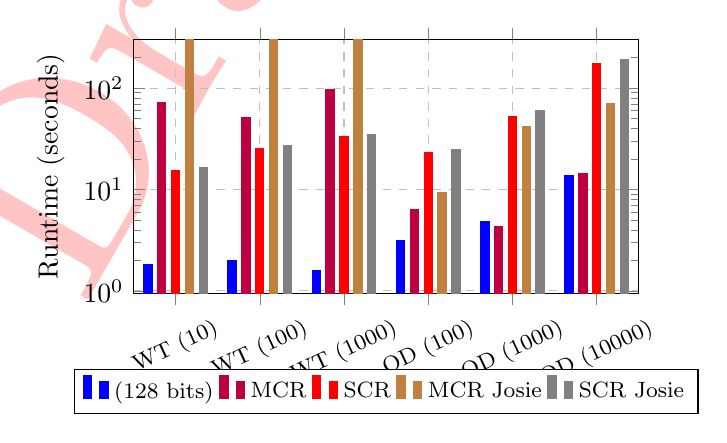
\begin{tikzpicture}
  \begin{groupplot}[xtick=data, ybar, enlarge x limits=0.1, symbolic x coords={WT (10), WT (100), WT (1000), OD (100), OD (1000), OD (10000)}, ymin = 0, group style={group size=1 by 1 , horizontal sep=.0cm}, height=4.8cm, width=8cm, ymax = 300, every node near coord/.append style={yshift=-0.21cm}, point meta=explicit symbolic, log origin=infty, xticklabel style={font=\footnotesize, rotate=25}, xmajorgrids=true, ymode = log, ytick={1, 10, 100, 1000, 10000},
    	ymajorgrids=true,grid style=dashed ]
    \nextgroupplot [ylabel={Runtime (seconds)}, 
    % legend style={legend columns=-1, at={(.95, 1)}}
    legend style={legend columns=5,at={(0.5,-0.3)},anchor=north,font=\footnotesize}
    , bar width=3pt]
    
    % \addplot[blue,fill] coordinates {(Webtable (10), 2.2) (Webtable (100), 5.4) (Webtable (1000), 4.9) (opendata (100), 2.2) (opendata (1000), 5.7) (opendata (10000), 32.5)};\addlegendentry{\hash (512 bits)};
    
    % \addplot[brown,fill] coordinates {(Webtable (10), 0) (Webtable (100), 0) (Webtable (1000), 0) (opendata (100), 4.9) (opendata (1000), 42.0) (opendata (10000), 64)}; \addlegendentry{Josie};
    
    % \addplot[red,fill] coordinates {(Webtable (10), 44.4) (Webtable (100), 55.2) (Webtable (1000), 59.9) (opendata (100), 29.8) (opendata (1000), 84.9) (opendata (10000), 503.1)}; \addlegendentry{SCI};
    
    
    % \addplot[blue,fill] coordinates {(Webtable (10), 1.0) (Webtable (100), 2.1) (Webtable (1000), 1.6) (opendata (100), .7) (opendata (1000), 2.7) (opendata (10000), 13)};\addlegendentry{\hash (512 bits)};
    
    % \addplot[brown,fill] coordinates {(Webtable (10), 0) (Webtable (100), 0) (Webtable (1000), 0) (opendata (100), 4.9) (opendata (1000), 42.0) (opendata (10000), 64)}; \addlegendentry{Multi-column Josie};
    
    % \addplot[red,fill] coordinates {(Webtable (10), 15.5) (Webtable (100), 25.4) (Webtable (1000), 33.5) (opendata (100), 22.9) (opendata (1000), 52.0  ) (opendata (10000), 175.6)}; \addlegendentry{SCI+Filtering};
    
    % \addplot[gray,fill] coordinates {(Webtable (10), 0) (Webtable (100), 0) (Webtable (1000), 0) (opendata (100), 26.16) (opendata (1000), 62.37) (opendata (10000), 196.08)}; \addlegendentry{Josie+Filtering};
    
    % \addplot[purple,fill] coordinates {(Webtable (10), 100.6) (Webtable (100), 82.70) (Webtable (1000), 140.8) (opendata (100), 12.8) (opendata (1000), 7.1) (opendata (10000), 19.60)}; \addlegendentry{Multi-column SCI};
    
    \addplot[blue,fill] coordinates {(WT (10), 1.8) (WT (100), 2.0) (WT (1000), 1.6) (OD (100),3.1) (OD (1000), 4.8) (OD (10000), 13.6)};\addlegendentry{\hash (128 bits)};
    
     \addplot[purple,fill] coordinates {(WT (10), 72.4) (WT (100), 51) (WT (1000), 97.6) (OD (100), 6.3) (OD (1000), 4.3) (OD (10000), 14.40)}; \addlegendentry{MCR};
    
    \addplot[red,fill] coordinates {(WT (10), 15.5) (WT (100), 25.4) (WT (1000), 33.5) (OD (100), 22.9) (OD (1000), 52.0) (OD (10000), 175.6)}; \addlegendentry{SCR};
    
    \addplot[brown,fill] coordinates {(WT (10), 300) (WT (100), 300) (WT (1000), 300)(OD (100), 9.4) (OD (1000), 42.0) (OD (10000), 71)}; \addlegendentry{MCR Josie};
    
    \addplot[gray,fill] coordinates {(WT (10), 16.6) (WT (100), 27.3) (WT (1000), 35) (OD (100), 24.7) (OD (1000), 60) (OD (10000), 191.8)}; \addlegendentry{SCR Josie};
    
  \end{groupplot}
\end{tikzpicture}
% \vspace{-.4cm}
\caption{Runtime comparison between \system and SCI.}
\label{fig:dxf_vs_mate_runtime}
%\vspace{-.2cm}
\end{figure}


%Here, we only report the runtime for the 512-bit version of \system.
%Later in this section, we also evaluate the system performance for hash arrays with varied sizes.
Figure~\ref{fig:dxf_vs_mate_runtime} shows the runtime comparison \system against SCR, MCR, and the corresponding JOSIE implementations in log scale.
Without the row filtering optimization of \system, the runtime for joinability calculation dominates the overall runtime.
The depicted runtime results for baselines include the time required to discover the multi-column joins in-memory on top of the state-of-the-art single-attribute joinable table discovery systems. 
Note that there is an additional fetching cost that is negligible, i.e.,~in the order of milliseconds when we use the in-memory implementation like state-of-the-art~\cite{zhu2019josie}. However, the fetching cost can vary between $1$ and $40$ seconds when the data and the index has to be retrieved from disk. This is the case for the DWTC, which cannot fit into memory. The depicted runtime does not contain the fetching time as it is the same for both approaches.
We observe that \system outperforms baseline systems in almost all experiments: it is up to $61x$, $13x$, $9x$, $22x$ faster than MCR, SCR, MCR Josie, and SCR Josie respectively.
%As a result, it can drop most of the non-joinable table rows before any further computation.
This experiment also shows that no other baseline constantly performs better than the other approaches. For instance, SCR-based approaches are slower than their corresponding MCR-based systems for open data queries but on the large webtable corpus they underperform. Note that MCR Josie for webtables did not terminate in $7$ days. The slower performance of the MCR approaches on webtable queries is because accessing the relevant PLs does not scale for the size of the webtable corpus. While MCR Josie performs similar to MCR in OD (100) its performance drops as the cardinality of the open data queries grows.
The size of the input dataset correlates with the runtime. This is expected because join columns with higher cardinality initially match more PL items in the index which again need to be fetched and filtered. 

In addition to the input table size, FPs play an important role in the number of comparisons and ultimately the runtime.
For instance, in case of SCR, although OD (1k) and WT (1k) have similar query table sizes, the OD (1k) queries lead to $35\%$ higher runtime than WT (1k). This increase in runtime is because of the large number of FPs for OD (1k) tables, i.e., $3M$ more FP rows compared to WT (1k).
%Moreover, For some query datasets, such as OD (10,000), the performance difference between \system and baselines is smaller, because the initial column filters already many of the FPs.
%On the other hand, for some datasets, such as WT (10), this performance gap is substantial because SCR retrieves over one orders of magnitude more FPs than \system. % 400 times more
\newline
\textbf{Summary.}
(i) \system is up to $100x$ faster than unary join discovery systems in discovering n-ary joins.
(ii) Performance gain of \system over SCR-based approaches depends on the number of FP rows.


\subsection{\hash VS. Baseline Hash Functions} \label{subsubsec:xash_vs_hashes}
Table~\ref{tab:dataset_runtime} depicts the runtime of \system with different hash functions, including the proposed \hash.
Note that all the competing hash functions benefit from all of \system's optimizations and only differ in the applied hash function during row filtering.

% \begin{table*}[]
%      \footnotesize
%     \centering
%     \caption{Runtime experiment (seconds). \colorbox[HTML]{A2EDFF}{blue} cells represent the experiments where the larger hash performs worse. \colorbox[HTML]{FFABA8}{Red} cells show the maximum performance gain of \system over BF.}
%     \label{tab:dataset_runtime}
% \begin{tabular}{r|r|r|r|r|rrr|rrr|rrr|rrr|rrr}
% \toprule
% \textit{\textbf{Dataset}} &
% \textit{\textbf{SCR}}&\textit{\textbf{\thead{MD5}}}&\textit{\textbf{{Murmur}}}&\textit{\textbf{{CityHash}}}&
%  \multicolumn{3}{c|}{\textit{\textbf{{SimHash}}}}& \multicolumn{3}{c|}{\textit{\textbf{{HT}}}}& \multicolumn{3}{c|}{\textit{\textbf{{BF}}}}& \multicolumn{3}{c|}{\textit{\textbf{{LHBF}}}}&  \multicolumn{3}{c}{\textit{\textbf{{\hash}}}}
%  \\

% &&\multicolumn{1}{c|}{\textbf{128}}&\multicolumn{1}{c|}{\textbf{128}}&\multicolumn{1}{c|}{\textbf{128}}&\multicolumn{1}{c}{\textbf{128}}&\multicolumn{1}{c}{\textbf{256}}&\multicolumn{1}{c|}{\textbf{512}}&\multicolumn{1}{c}{\textbf{128}}&\multicolumn{1}{c}{\textbf{256}}&\multicolumn{1}{c|}{\textbf{512}}&\multicolumn{1}{c}{\textbf{128}}&\multicolumn{1}{c}{\textbf{256}}&\multicolumn{1}{c|}{\textbf{512}}&\multicolumn{1}{c}{\textbf{128}}&\multicolumn{1}{c}{\textbf{256}}&\multicolumn{1}{c|}{\textbf{512}}&\multicolumn{1}{c}{\textbf{128}}&\multicolumn{1}{c}{\textbf{256}}&\multicolumn{1}{c}{\textbf{512}}\\
% \toprule
% WT (10) & 15.5 & 8.6 & 8.4 & 8.6 & {7.0}&\colorbox[HTML]{A2EDFF}{8.0}& 4.1 & {4.3}&\colorbox[HTML]{A2EDFF}{6.3}& 3.1 & {2.5}&\colorbox[HTML]{A2EDFF}{3.0}& 1.6  & {2.9}&\colorbox[HTML]{A2EDFF}{3.2}& 2.1  & \textbf{1.0}&\textbf{1.0}&\textbf{0.7}  \\

% WT (100) & 25.4 & 15.7 & 15.2 & 15.7 & 13.7&8.5&6.1 & {9.6}&\colorbox[HTML]{A2EDFF}{10.2}&4.1 & {4.9}&\colorbox[HTML]{A2EDFF}{5.3}&2.8 &{5.7} &{3.5}&\colorbox[HTML]{A2EDFF}{4.4}& {\textbf{1.6}}&\colorbox[HTML]{A2EDFF}{\textbf{1.8}}&\textbf{1.2}\\

% WT (1000) & 33.5 & 20.8 & 20.5 & 20.4 & 17.2&10.2&6.9 & {13.7}& \colorbox[HTML]{A2EDFF}{13.9}&5.3 & 5.7&5.5&{2.4} & 7.5&{4.1}&\colorbox[HTML]{A2EDFF}{4.6} & \textbf{1.6}&\textbf{1.5}&{\textbf{1.2}} \\

% \toprule

% OD (100) & 22.9 & {22.0} & 21.7 & 21.9 & {20.8}&\colorbox[HTML]{A2EDFF}{22.8}&{21.1} & 7.8&6.7&4.5 & 4.2&2.6&\colorbox[HTML]{FFABA8}{1.8} & 6.2 &4.8&2.9& \textbf{3.5}&\textbf{1.0}&\colorbox[HTML]{FFABA8}{\textbf{0.7}}\\

% OD (1000) & 52.0 & 50.4 & 49.8 & 51.1 & {47.9}&\colorbox[HTML]{A2EDFF}{49.4}&43.95 & 17.1&16.5&13.2 & 10.9&6.5&4.8 & 15.5&12.0&8.3 & \textbf{7.0}&\textbf{3.1}&\textbf{2.7} \\

% OD (10000) & 175.6 & {137.4} & {130.2} & {131.9} & {123.9}&120.2&99.4 & 44.6&44.6&33.5 & 28.2&18.8&15.1 & 36.3&29.3&22.2 & \textbf{18}&\textbf{13.3}&\textbf{13}\\
% \toprule
% Kaggle & 297.0 & 97.6 &104.2&104.4&{76.6}&57.3&41.0&34.8&30.3&25.9&19.7&14.8&13.1 & 37.8&27.1&21.8&\textbf{15.2}&\textbf{12.0}&{\textbf{12.3}}\\
% \toprule
% School & 873.6 & 772.7 & 772.9 & 742.8 & 593.7&444.0&307.2 & 54.3&38.3&31.0 & 24.2&19.0& 19.0 & 33.8&25.3&22.7 &\textbf{20.0}&\textbf{17.9}&\textbf{17.6}\\
% \end{tabular}
% \end{table*}



\begin{table*}[]
     \footnotesize
    \centering
    \caption{Runtime experiment (seconds). \colorbox[HTML]{A2EDFF}{blue} cells represent the experiments where the larger hash performs worse. \colorbox[HTML]{FFABA8}{Red} cells show the maximum performance gain of \system over BF.}
    % \vspace{-.2cm}
    \label{tab:dataset_runtime}
\begin{tabular}{r|r|r|r|r|rrr|rrr|rrr|rrr|rrr}
%\toprule
\textit{\textbf{Dataset}} &
\textit{\textbf{SCR}}&\textit{\textbf{\thead{MD5}}}&\textit{\textbf{{Murmur}}}&\textit{\textbf{{City}}}&
 \multicolumn{3}{c|}{\textit{\textbf{{SimHash}}}}& \multicolumn{3}{c|}{\textit{\textbf{{HT}}}}& \multicolumn{3}{c|}{\textit{\textbf{{BF}}}}& \multicolumn{3}{c|}{\textit{\textbf{{LHBF}}}}&  \multicolumn{3}{c}{\textit{\textbf{{\hash}}}}
 \\

&&\multicolumn{1}{c|}{\textbf{128}}&\multicolumn{1}{c|}{\textbf{128}}&\multicolumn{1}{c|}{\textbf{128}}&\multicolumn{1}{c}{\textbf{128}}&\multicolumn{1}{c}{\textbf{256}}&\multicolumn{1}{c|}{\textbf{512}}&\multicolumn{1}{c}{\textbf{128}}&\multicolumn{1}{c}{\textbf{256}}&\multicolumn{1}{c|}{\textbf{512}}&\multicolumn{1}{c}{\textbf{128}}&\multicolumn{1}{c}{\textbf{256}}&\multicolumn{1}{c|}{\textbf{512}}&\multicolumn{1}{c}{\textbf{128}}&\multicolumn{1}{c}{\textbf{256}}&\multicolumn{1}{c|}{\textbf{512}}&\multicolumn{1}{c}{\textbf{128}}&\multicolumn{1}{c}{\textbf{256}}&\multicolumn{1}{c}{\textbf{512}}\\
\toprule
WT (10) & 20.6 & 12.5 & 12.6 & 12.6 & 11.1 & 10.1 & \colorbox[HTML]{A2EDFF}{12.5} & 6.4 & \colorbox[HTML]{A2EDFF}{7.3} & \colorbox[HTML]{A2EDFF}{7.6} & 4.2 & 4.2 & \colorbox[HTML]{A2EDFF}{10.3} & 4.1 & 3.6 & 2.2 & \textbf{1.8} & \textbf{1.5} & \textbf{1.4} \\
WT (100) & 24.5 & 15.3 & 14.8 & 15.3 & 13.4 & 8.5 & \colorbox[HTML]{A2EDFF}{17.2} & 9.5 & \colorbox[HTML]{A2EDFF}{10.1} & \colorbox[HTML]{A2EDFF}{12.4} & 4.7 & \colorbox[HTML]{A2EDFF}{5.0} & \colorbox[HTML]{A2EDFF}{16.8} & 5.6 & 3.6 & \colorbox[HTML]{A2EDFF}{4.2} & \textbf{1.6} & \colorbox[HTML]{A2EDFF}{\textbf{1.8}} & \colorbox[HTML]{A2EDFF}{\textbf{2.0}}\\
WT (1k) & 32.7 & 20.2 & 19.8 & 19.8 & 16.3 & 10.0 & \colorbox[HTML]{A2EDFF}{17.0} & 13.4 & \colorbox[HTML]{A2EDFF}{13.8} & 13.4 & 5.6 & 5.5 & \colorbox[HTML]{FFABA8}{16.7} & 7.6 & 4.1 & \colorbox[HTML]{A2EDFF}{4.6} & \textbf{1.6} & \textbf{1.5} & \colorbox[HTML]{FFABA8}{\textbf{1.6}}\\
\toprule
OD (100) & 247.6 & 212.1 & 224.2 & 194.5 & 102.9 & 69.1 & 56.5 & 24.0 & 16.4 & 10.8 & 11.0 & 4.8 & 3.4 & 30.1 & 9.5 & 8.3 & \textbf{6.5} & \textbf{3.5} & \textbf{3.}1\\
OD (1k) & 165.8 & 146.8 & 152.3 & 138.6 & 90.0 & 73.6 & 62.6 & 25.4 & 21.6 & 16.5 & 14.4 & 7.6 & 5.6 & 39.2 & 11.3 & \colorbox[HTML]{A2EDFF}{13.0} & \textbf{8.7} & \textbf{4.5} & \colorbox[HTML]{A2EDFF}{\textbf{4.8}}\\
OD (10k) & 256.7 & 203.9 & 202.1 & 190.6 & 145.6 & 127.0 & 103.5 & 49.6 & 44.0 & 31.9 & 27.7 & 17.8 & 14.3 & 79.2 & 27.0 & 21.8 & \textbf{17.6} & \textbf{13.4} & \colorbox[HTML]{A2EDFF}{\textbf{13.6}}\\
\toprule
Kaggle & 297.0 & 97.6 &104.2&104.4&{76.6}&57.3&41.0&34.8&30.3&25.9&19.7&14.8&13.1 & 37.8&27.1&21.8&\textbf{15.2}&\textbf{12.0}&{\textbf{12.3}}\\
\toprule
School & 873.6 & 772.7 & 772.9 & 742.8 & 593.7&444.0&307.2 & 54.3&38.3&31.0 & 24.2&19.0& 19.0 & 33.8&25.3&22.7 &\textbf{20.0}&\textbf{17.9}&\textbf{17.6}\\
\end{tabular}
\end{table*}
% \begin{table*}[]
%     % \vspace{-.2cm}
%     \footnotesize
%     \centering
%     \caption{Precision experiment.}
%         \vspace{-.1cm}
%     \label{tab:dataset_precision}
% \begin{tabular}{r|rrrrrrr|rrrrr}
% \toprule
% \textit{\textbf{Dataset}} & \textit{\textbf{\thead{MD5\\Murmur\\(128)}}}&\textit{\textbf{\thead{CityHash \\ (128)}}} & \textit{\textbf{\thead{SimHash \\(128)}}}& \textit{\textbf{\thead{HT \\ (128)}}}& \textit{\textbf{\thead{BF \\(128)}}}&\textit{\textbf{\thead{LHBF \\(128)}}}& \textit{\textbf{\thead{\hash \\ (128)}}}&
% \textit{\textbf{\thead{SimHash \\(512)}}}&\textit{\textbf{\thead{HT \\ (512)}}}& \textit{\textbf{\thead{BF \\(512)}}}&\textit{\textbf{\thead{LHBF \\(512)}}}& \textit{\textbf{\thead{\hash \\ (512)}}}\\ \toprule

% WT (10) & 0.28$\pm$0.40 & 0.28$\pm$0.40 & 0.30$\pm$0.41 & 0.34$\pm$0.43 & 0.45$\pm$0.46 & 0.44$\pm$0.44 & \textbf{0.58$\pm$0.46} & 0.35$\pm$0.43 & 0.43$\pm$0.46 & 0.62$\pm$0.45 &  0.61$\pm$0.46 & \textbf{0.94$\pm$0.20}\\
% WT (100) & 0.26$\pm$0.40 & 0.27$\pm$0.40 & 0.27$\pm$0.40 & 0.34$\pm$0.41 & 0.45$\pm$0.44 &  0.45$\pm$0.43 & \textbf{0.60$\pm$0.44} & 0.33$\pm$0.42 & 0.45$\pm$0.43 & 0.69$\pm$0.42  &  0.60$\pm$0.45 & \textbf{0.95$\pm$0.20}\\
% WT (1000) & 0.22$\pm$0.35 & 0.22$\pm$0.35 & 0.24$\pm$0.35 & 0.37$\pm$0.37 & 0.56$\pm$0.40 &  0.51$\pm$0.39 & \textbf{0.76$\pm$0.35} & 0.34$\pm$0.39 & 0.53$\pm$0.39 & 0.79$\pm$0.35 &  0.75$\pm$0.37 & \textbf{0.98$\pm$0.10}\\
% \toprule
% OD (100) & 0.36$\pm$0.42 & 0.36$\pm$0.42 & 0.37$\pm$0.42 & 0.54$\pm$0.40 & 0.66$\pm$0.41 &  0.62$\pm$0.41 & \textbf{0.77$\pm$0.38} & 0.39$\pm$0.41 & 0.67$\pm$0.40 & 0.86$\pm$0.30 &  0.78$\pm$0.35 & \textbf{0.97$\pm$0.13}\\
% OD (1000) & 0.37$\pm$0.43 & 0.37$\pm$0.43 & 0.37$\pm$0.42 & 0.53$\pm$0.41 & 0.65$\pm$0.40 &  0.63$\pm$0.42 & \textbf{0.75$\pm$0.37} & 0.46$\pm$0.42 & 0.68$\pm$0.41 & 0.90$\pm$0.26 &  0.76$\pm$0.36 & \textbf{0.97$\pm$0.15}\\
% OD (10000) & 0.37$\pm$0.43 & 0.37$\pm$0.43 & 0.37$\pm$0.42 & 0.53$\pm$0.41 & 0.65$\pm$0.40 &  0.50$\pm$0.40 & \textbf{0.75$\pm$0.37} & 0.46$\pm$0.42 & 0.66$\pm$0.41 & 0.90$\pm$0.26 &  0.72$\pm$0.36 & \textbf{0.97$\pm$0.15}\\
% \toprule
% Kaggle & 0.09$\pm$0.18&   0.09$\pm$0.17&   0.12$\pm$0.21&  0.25$\pm$0.31&  0.40$\pm$0.41&  0.33$\pm$0.34 &  \textbf{0.64$\pm$0.34}&   0.20$\pm$0.31&    0.44$\pm$0.37&    0.64$\pm$0.38 & 0.63$\pm$0.36 & \textbf{0.93$\pm$0.10}\\
% \toprule
% School & 0.00$\pm$0.00&   0.00$\pm$0.00&   0.00$\pm$0.00&  0.01$\pm$0.01&  0.07$\pm$0.03&  0.02$\pm$0.01 &  \textbf{0.43$\pm$0.11}&   0.00$\pm$0.00&    0.03$\pm$0.02&    \textbf{1.00$\pm$0.00} & 0.24$\pm$0.08 & 0.96$\pm$0.02\\
% \toprule
% Average &    0.24$\pm$0.33&   0.25$\pm$0.33&   0.26$\pm$0.33&  0.36$\pm$0.34&  0.49$\pm$0.37&  0.44$\pm$0.36 &  \textbf{0.66$\pm$0.35}&       0.32$\pm$0.35&    0.49$\pm$0.36&    0.80$\pm$0.30 & 0.64$\pm$0.35 & \textbf{0.96$\pm$0.13} \\

% \end{tabular}
% \end{table*}



% \begin{table*}[]
%     % \vspace{-.2cm}
%     \footnotesize
%     \centering
%     \caption{Precision experiment.}
%         \vspace{-.1cm}
%     \label{tab:dataset_precision}
% \begin{tabular}{r|rrrrrrr|rrrrr}
% \toprule
% \textit{\textbf{Dataset}} & \textit{\textbf{\thead{MD5\\Murmur\\(128)}}}&\textit{\textbf{\thead{CityHash \\ (128)}}} & \textit{\textbf{\thead{SimHash \\(128)}}}& \textit{\textbf{\thead{HT \\ (128)}}}& \textit{\textbf{\thead{BF \\(128)}}}&\textit{\textbf{\thead{LHBF \\(128)}}}& \textit{\textbf{\thead{\hash \\ (128)}}}&
% \textit{\textbf{\thead{SimHash \\(512)}}}&\textit{\textbf{\thead{HT \\ (512)}}}& \textit{\textbf{\thead{BF \\(512)}}}&\textit{\textbf{\thead{LHBF \\(512)}}}& \textit{\textbf{\thead{\hash \\ (512)}}}\\ \toprule

% WT (10) & 0.27$\pm$0.39 & 0.25$\pm$0.38 & 0.28$\pm$0.40 & 0.34$\pm$0.43 & 0.44$\pm$0.46 & 0.44$\pm$0.45 & \textbf{0.57$\pm$0.46} & 0.31$\pm$0.42 & 0.28$\pm$0.43 & 0.40$\pm$0.43 & 0.61$\pm$0.46 & \textbf{0.88$\pm$0.26}   \\
% WT (100) & 0.27$\pm$0.40 & 0.27$\pm$0.40 & 0.27$\pm$0.40 & 0.34$\pm$0.41 & 0.46$\pm$0.44 & 0.45$\pm$0.43 & \textbf{0.61$\pm$0.43} & 0.27$\pm$0.39 & 0.38$\pm$0.41 & 0.34$\pm$0.41 & 0.63$\pm$0.44 & \textbf{0.93$\pm$0.22}   \\
% WT (1000) & 0.24$\pm$0.36 & 0.24$\pm$0.36 & 0.25$\pm$0.37 &  0.40$\pm$0.37 & 0.59$\pm$0.39 & 0.52$\pm$0.38 & \textbf{0.77$\pm$0.34} &  0.28$\pm$0.35 & 0.42$\pm$0.36 & 0.32$\pm$0.35 & 0.78$\pm$0.33 & \textbf{0.98$\pm$0.10} \\
% \toprule
% OD (100) & 0.27$\pm$0.38 & 0.28$\pm$0.39 & 0.28$\pm$0.38 & 0.43$\pm$0.40 & \textbf{0.56$\pm$0.41} & 0.45$\pm$0.43 & 0.52$\pm$0.41 & 0.32$\pm$0.41 & 0.55$\pm$0.41 & 0.79$\pm$0.34 & 0.67$\pm$0.35 & \textbf{0.80$\pm$0.34}   \\
% OD (1000) & 0.32$\pm$0.40 & 0.32$\pm$0.40 & 0.32$\pm$0.39 & 0.47$\pm$0.40 & \textbf{0.61$\pm$0.40} & 0.44$\pm$0.34 & 0.53$\pm$0.41 & 0.41$\pm$0.41 & 0.59$\pm$0.41 & 0.85$\pm$0.28 & 0.63$\pm$0.39 & \textbf{0.86$\pm$0.28}   \\
% OD (10000) & 0.27$\pm$0.38 & 0.28$\pm$0.38 & 0.28$\pm$0.37 & 0.42$\pm$0.39 & \textbf{0.59$\pm$0.40} & 0.40$\pm$0.42 & 0.52$\pm$0.42 & 0.34$\pm$0.39 & 0.56$\pm$0.39 & \textbf{0.87$\pm$0.27} & 0.66$\pm$0.40 & 0.82$\pm$0.32   \\
% \toprule
% School & 0.00$\pm$0.00&   0.00$\pm$0.00&   0.00$\pm$0.00&  0.01$\pm$0.01&  0.07$\pm$0.03&  0.02$\pm$0.01 &  \textbf{0.43$\pm$0.11}&   0.00$\pm$0.00&    0.03$\pm$0.02&    \textbf{1.00$\pm$0.00} & 0.24$\pm$0.08 & 0.96$\pm$0.02\\
% \toprule
% Kaggle & 0.09$\pm$0.18&   0.09$\pm$0.17&   0.12$\pm$0.21&  0.25$\pm$0.31&  0.40$\pm$0.41&  0.33$\pm$0.34 &  \textbf{0.64$\pm$0.34}&   0.20$\pm$0.31&    0.44$\pm$0.37&    0.64$\pm$0.38 & 0.63$\pm$0.36 & \textbf{0.93$\pm$0.10}\\
% \toprule
% Average &    0.24$\pm$0.33&   0.25$\pm$0.33&   0.26$\pm$0.33&  0.36$\pm$0.34&  0.49$\pm$0.37&  0.44$\pm$0.36 &  \textbf{0.66$\pm$0.35}&       0.32$\pm$0.35&    0.49$\pm$0.36&    0.80$\pm$0.30 & 0.64$\pm$0.35 & \textbf{0.96$\pm$0.13} \\

% \end{tabular}
% \end{table*}






\begin{table*}[]
     \footnotesize
    \centering
    \caption{Precision experiment.}
    % \vspace{-.2cm}
    \label{tab:dataset_precision}
\begin{tabular}{r|c|c|rr|rr|rr|rr|rr}
%\toprule
\textit{\textbf{Dataset}} &
\textit{\textbf{\thead{MD5}}}&\textit{\textbf{{CityHash}}}&
 \multicolumn{2}{c|}{\textit{\textbf{{SimHash}}}}& \multicolumn{2}{c|}{\textit{\textbf{{HT}}}}& \multicolumn{2}{c|}{\textit{\textbf{{BF}}}}& \multicolumn{2}{c|}{\textit{\textbf{{LHBF}}}}&  \multicolumn{2}{c}{\textit{\textbf{{\hash}}}}
 \\

&\multicolumn{1}{c|}{\textbf{128}}&\multicolumn{1}{c|}{\textbf{128}}&\multicolumn{1}{c}{\textbf{128}}&\multicolumn{1}{c|}{\textbf{512}}&\multicolumn{1}{c}{\textbf{128}}&\multicolumn{1}{c|}{\textbf{512}}&\multicolumn{1}{c}{\textbf{128}}&\multicolumn{1}{c|}{\textbf{512}}&\multicolumn{1}{c}{\textbf{128}}&\multicolumn{1}{c|}{\textbf{512}}&\multicolumn{1}{c}{\textbf{128}}&\multicolumn{1}{c}{\textbf{512}}\\
\toprule
WT (10) & 0.27$\pm$0.39 & 0.25$\pm$0.38 & 0.28$\pm$0.40 &0.31$\pm$0.42& 0.34$\pm$0.43 &0.28$\pm$0.43 & 0.44$\pm$0.46 &0.40$\pm$0.43 & 0.44$\pm$0.45 & 0.61$\pm$0.46& \textbf{0.57$\pm$0.46} & \textbf{0.88$\pm$0.26}   \\
WT (100) & 0.27$\pm$0.40 & 0.27$\pm$0.40 & 0.27$\pm$0.40 &0.27$\pm$0.39 & 0.34$\pm$0.41 &0.38$\pm$0.41 & 0.46$\pm$0.44 &0.34$\pm$0.41  & 0.45$\pm$0.43 & 0.63$\pm$0.44& \textbf{0.61$\pm$0.43} &\textbf{0.93$\pm$0.22} \\
WT (1k) & 0.24$\pm$0.36 & 0.24$\pm$0.36 & 0.25$\pm$0.37 & 0.28$\pm$0.35 &  0.40$\pm$0.37 &0.42$\pm$0.36 &  0.59$\pm$0.39 & 0.32$\pm$0.35&  0.52$\pm$0.38  &0.78$\pm$0.33 & \textbf{0.77$\pm$0.34} &\textbf{0.98$\pm$0.10}  \\
\toprule
OD (100) & 0.27$\pm$0.38 & 0.28$\pm$0.39 & 0.28$\pm$0.38 &0.32$\pm$0.41 & 0.43$\pm$0.40 &0.55$\pm$0.41 & \textbf{0.56$\pm$0.41} & 0.79$\pm$0.34& 0.45$\pm$0.43 &0.67$\pm$0.35 & 0.52$\pm$0.41 & \textbf{0.80$\pm$0.34}   \\
OD (1k) & 0.32$\pm$0.40 & 0.32$\pm$0.40 & 0.32$\pm$0.39 &0.41$\pm$0.41 & 0.47$\pm$0.40 &0.59$\pm$0.41 & \textbf{0.61$\pm$0.40} &0.85$\pm$0.28 & 0.44$\pm$0.34 & 0.63$\pm$0.39 & 0.53$\pm$0.41 & \textbf{0.86$\pm$0.28}   \\
OD (10k) & 0.27$\pm$0.38 & 0.28$\pm$0.38 & 0.28$\pm$0.37 & 0.34$\pm$0.39& 0.42$\pm$0.39 &0.56$\pm$0.39 & \textbf{0.59$\pm$0.40} & \textbf{0.87$\pm$0.27}& 0.40$\pm$0.42 & 0.66$\pm$0.40& 0.52$\pm$0.42 & 0.82$\pm$0.32   \\
\toprule
School & 0.00$\pm$0.00&   0.00$\pm$0.00&   0.00$\pm$0.00 & 0.00$\pm$0.00 & 0.01$\pm$0.01& 0.03$\pm$0.02 & 0.07$\pm$0.03&  \textbf{1.00$\pm$0.00} & 0.02$\pm$0.01 & 0.24$\pm$0.08 & \textbf{0.43$\pm$0.11}& 0.96$\pm$0.02\\
\toprule
Kaggle & 0.09$\pm$0.18&   0.09$\pm$0.17&   0.12$\pm$0.21 &  0.20$\pm$0.31 &  0.25$\pm$0.31& 0.44$\pm$0.37 &  0.40$\pm$0.41&  0.64$\pm$0.38 &  0.33$\pm$0.34 & 0.63$\pm$0.36 &  \textbf{0.64$\pm$0.34}& \textbf{0.93$\pm$0.10}\\
\toprule
Average &    0.22$\pm$0.31&   0.22$\pm$0.31&   0.23$\pm$0.32&  0.27$\pm$0.34&  0.33$\pm$0.34&  0.41$\pm$0.35 &  0.47$\pm$0.37&       0.65$\pm$0.31&    0.38$\pm$0.35&    0.61$\pm$0.35 & \textbf{0.57$\pm$0.37} & \textbf{0.90$\pm$0.21} \\
\end{tabular}
\end{table*}
In Table~\ref{tab:dataset_runtime}, we highlight the best performing approach of each row and hash size in \textbf{bold} font.
We observe that \system with \hash outperforms all the other baselines on all of the queries.
%\hash leverages simple syntactic information of the cell values to generate distinguishable index elements. 
\system + \hash can be up to $10x$ faster than \system + BF, which is the second most efficient baseline on average.
The cells showing this speedup are highlighted with \colorbox[HTML]{FFABA8}{red}.
BF's under-performance is rooted in its higher collision rate compared to \hash. Besides, by checking the length attribute that we use in \hash to generate the hash results, we can drop many of the non-joinable rows without evaluating all the bits in the super keys. This feature gives \system a superiority over BF in runtime even in the cases with similar or lower FP rates.
Another interesting insight is that \system + BF is faster than \system + HT in most of the cases and this is because BF is able to leverage more bits in the hash space to encode the join keys than a hash table that leverages only a single bit to hash each key value.%A single bit can only generate a limited number of unique hash values, e.g., 128 different hash values in 128-bit hash space, therefore, in the best case, $\frac{1}{128}$ of the single hashes will lead to collision, i.e., the same hash value. 
Table~\ref{tab:dataset_runtime} shows that \hash performs also better than LHBF in all of the cases. LHBF leverages fewer hash functions in comparison to BF with statistically similar FP probability. However, similar to HT, fewer hashing does not necessarily lead to a better performance in discovering the joinable tables. In our experiments LHBF only performs better on larger hash sizes for webtable queries, but in the remaining cases, LHBF is less efficient than BF.

The results also show that although super keys based on the standard hash functions, MD5, CityHash, SimHash, and Murmur, lead to overall performance gains over the naive SCR approach, all of them clearly fall behind \hash.
This is because they are not optimized to identify subset relationships that we encode via bitwise OR masking. They generate too many 1 bits (on average $50\%$) in the hash results, which leads to a higher number of FPs.
Thus, if a table contains six columns the aggregation of six hash results will on average turn $98\%$ of the super key to 1s, which would make the super key highly ineffective in masking.

%MD5, CityHash, SimHash, and Murmur lead to a very similar performance to SCR specially in open data and school experiments. This performance drop is because the row filtering overhead is almost as high as the runtime benefit from the row filtering.

Further, the experiments show that in most of the cases, a larger hash size (512 bits) leads to a faster join discovery than the smaller versions. However, in cases such as WT (100) and Simhash, the larger hash size results in slower discovery. The experiments that lead to slower runtime compared to their smaller hash size are marked as \colorbox[HTML]{A2EDFF}{blue} cells. 
When the FP rate is similar for two hash sizes, the approach with the larger hash size will result in similar or higher runtime. 
This is because the bit-wise OR operation is more expensive for larger hash values.
For instance, for WT (100) query tables and SimHash, the difference between the FP rate is almost zero, therefore, the runtime overhead of 512-bit hash causes worse performance.
In the more common case that a larger hash size reduces the number of FPs the resulting runtime is also lower.
For example, for the OD (100) datasets, the larger hash size for \hash results in $85\%$ fewer FPs on average, leading to $48\%$ speed-up.

Finally, we also observed that \system can indeed find interesting joinable tables based on composite keys. 
%Similarly, we observe that using composite keys we can find interesting tables for almost any dataset.  
% As another example, the most joinable table to the \textit{Page View} dataset~\cite{base_pageview} with query columns <``Name'', ``Country''>, which contains the information about Wikipedia pages of people, reveals the birth/death date of the people in the given countries. 
Searching for the top joinable tables to Kaggle Movie dataset based on a single-column join and ``Movie Title'' key columns, none of the top-10 tables contains more than one additional column, containing float numbers. However, using our multi-column join discovery approach and query columns <``Director name'', ``Movie Title''>, we obtain a table with 8 columns worth of information, including the plot of the movie, actor names, etc.
For the \textit{Kaggle Airline} dataset with join keys ``Airline name'' and ``Country'' \system obtains a table representing the airports in which the airlines operate flights in the given countries. 

\noindent\textbf{Summary.}
(i)~The syntactic feature extraction in \hash leads to a faster multi-attribute join discovery compared to the baselines;
(ii)~the standard hash functions are not ideal for n-ary joins due to their uniform distribution property that results in too many 1 bits; and
(iii)~ larger hash sizes result in higher calculation overhead.

\subsection{FP Rate}\label{subsubsection:fp}
%We now delve into more details regarding the FP rates.
There is a direct relationship between the table discovery runtime and the FP rate of the hash function used.
We measure the precision as the ratio of true positives (TP) over both TPs and FPs: $precision = \frac{TP}{TP + FP}$. Precision normalizes the TP-rate across datasets.

Table~\ref{tab:dataset_precision} shows the results of this experiment. Due to space reasons in this experiment, we only show the results for $128$- and $512$-bit hash sizes. Note that we observe the same trends as the other hash sizes.
Like runtime, precision increases with larger hash sizes in most of the cases. This is due to the fact that hash functions can scatter the values in a larger range and this leads to lower collision rate between super keys.
On average, \system + \hash achieves the highest precision compared to all the other approaches both in 128- and 512-bit hash spaces. \hash achieves up to $25\%$ higher precision than BF. 
% \hash maps the character and length features of the cell values to hash bits and rotates them based on the length. This removes the random overlap between the hashes. 
However, in five cases, BF outperforms \hash. In these experiments the difference between BF and \hash is only $4\%$.
\system's runtime superiority regardless of its precision is because of the design of \hash: the length feature of the cell value is located on the left-most segment of the array. Thus, the bit-wise OR operation can skip a table row before even getting to the character features of the cell values ensuring that this happens in the very first bit-segment of the hash. If the length of the key value has never appeared in the candidate row, \system moves to the next row.
In baseline approaches, such as BF, the 0-bits are randomly scattered. Therefore, step-wise filtering might take longer to find the contradicting bits.
% For query tables, such as WT (1k), \hash leads to distinctively high precision with 128 bits. 
%\hash achieves up to $25\%$ higher precision than BF. 
\hash displays the smallest standard deviation showing its robustness in achieving high precision.
In general, the precision achieved by LHBF is consistent with its runtime performance compared to the BF approach. LHBF achieves higher precision and ultimately, lower runtime for webtable queries with $512$-bit hash sizes but in the remaining experiments BF outperforms LHBF.
%As observed before, the SimHash function performs better than the other remaining hash functions. %CityHash performs very similarly to Murmur and MD5 except on WT (100), OD (100), and OD (10k), where CityHash gains up to $2\%$ more precision.
% As the precision experiments show, BF performs better than \hash in a single case of school query tables and $512$-bits hash size. However, due to the special hash design in \hash and the segmentation of the hash array, the evaluation process in \hash is much faster than BF. In \hash, a large portion of the FPs are pruned by only checking the length bits. This optimization prevents from checking all the remaining bits and leads to faster join discovery.

\noindent\textbf{Summary.}
(i) The precision of an approach correlates with its runtime.
(iii) The segmentation of bits in \hash leads to faster join discovery even in cases where precision rates are similar.

\subsection{\system In Depth}
\subsubsection{Top-$k$.}
% \begin{figure}[t!]
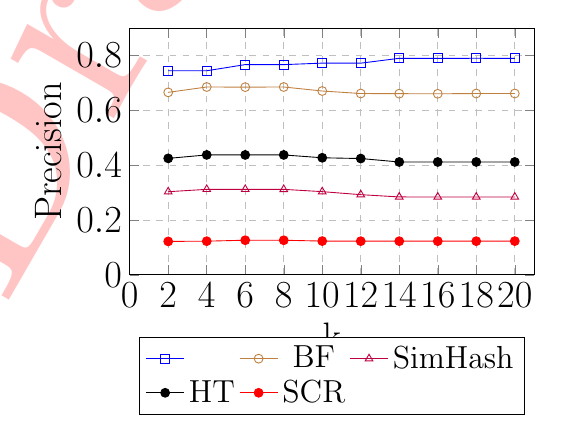
\begin{tikzpicture}[scale=0.8]
  \begin{groupplot}
    \nextgroupplot [
    	xlabel={k},
    	ylabel={Precision},
    	label style={font=\LARGE},
    	tick label style={font=\LARGE},
    	legend style={legend columns=3,at={(0.5,-0.25)},anchor=north,font=\Large},
    	width = 8cm,
    	height = 5.5cm,
    	xmin=0,
    	xmax=21,
    	ymin= 0,
    	ymax=.9,
    % 	ymode=log,
    	xtick={0, 2, 4, 6, 8, 10, 12, 14, 16, 18, 20},
    	ytick={0, .2, .4, .6, .8},
    	xmajorgrids=true,
    	ymajorgrids=true,
    	grid style=dashed]
    % 	\addplot[color=orange,mark=x] coordinates{(1,20588)(2,21069)(3,22225)(4,28451)(5,33406)(6,36650)(7,38444)(8,39346)(9,41242)(10,42847)(11,45166)(12,48807)(13,51618)(14,55643)(15,57868)(16,58111)(17,59849)(18,60661)(19,61591)(20,61883)}; \addlegendentry{True positives}
    	\addplot[color=blue,mark=square] coordinates{(2, 0.7444244234644304)(4, 0.7444460986518573)(6, 0.766964592170994)(8, 0.7668418665646705)(10, 0.7723498169274685)(12, 0.7721850123943121)(14, 0.789895797886049)(16, 0.7898665438117544)(18, 0.7899121864602451)(20, 0.7898665438117544)
}; \addlegendentry{\hash}
    	\addplot[color=brown,mark=o] coordinates{(2, 0.6657185337122508)(4, 0.6852987283763192)(6, 0.6847869632839787)(8, 0.6853100974388263)(10, 0.6706663366294509)(12, 0.6615030786875513)(14, 0.6609914966790925)(16, 0.6605009207276907)(18, 0.6615030239812544)(20, 0.6615030968085653)
}; \addlegendentry{BF}
    % 	\addplot[color=green,mark=otimes] coordinates{(1, 0.008487964801414276)(2, 0.00867506847329665)(3, 0.009056228892568881)(4, 0.011118979450347002)(5, 0.010706217432424333)(6, 0.010493747272771001)(7, 0.01087875580809653)(8, 0.010654525140330435)(9, 0.010256007269375988)(10, 0.010313630953168985)(11, 0.009810088365946748)(12, 0.009603656106980404)(13, 0.009668111695178587)(14, 0.010120234047804433)(15, 0.010479001253467317)(16, 0.010491242012774505)(17, 0.010487978665500265)(18, 0.01042295610506084)(19, 0.010553417433743212)(20, 0.010502225759753715)}; \addlegendentry{MD5}
    	\addplot[color=purple,mark=triangle] coordinates{(2, 0.30345662577661975)(4, 0.312138456555909)(6, 0.31220590396905923)(8, 0.31208672045033997)(10, 0.3036917898770219)(12, 0.2926698617018144)(14, 0.28438747405412956)(16, 0.2843694657737292)(18, 0.2843812923475462)(20, 0.28436718822604207)
}; \addlegendentry{SimHash}
        \addplot[color=black,mark=*] coordinates{(2, 0.42501046760605)(4, 0.43763678480021895)(6, 0.4375524593109754)(8, 0.43756087888715633)(10, 0.42717674533780864)(12, 0.4244305492112715)(14, 0.41187722681746775)(16, 0.411916505462486)(18, 0.4119544603091702)(20, 0.4118983532382111)
}; \addlegendentry{HT}
        \addplot[color=red,mark=*] coordinates{(2, 0.12227078467022626)(4, 0.12308378688197472)(6, 0.12659158889930547)(8, 0.12646800973130415)(10, 0.12348312509596455)(12, 0.12307493167176285)(14, 0.12310921932932725)(16, 0.12315553533822131)(18, 0.123103309723566)(20, 0.12328776753409271)
}; \addlegendentry{SCR}
		
  \end{groupplot}
\end{tikzpicture}
\caption{topk experiment.}
\label{fig:topk}
\end{figure}
The number of top-$k$ joinable tables changes the stopping criteria of the system (see table filtering step in Section~\ref{sec:index_applicaiton}).
Larger $k$ requires more tables to be evaluated.
In this experiment, we measure the precision of \system with different hash functions and vary $k$ from $2$ to $20$.
We ran the experiment with the WT (100) datasets as the input dataset against the DWTC corpus.
Other variables, such as key columns, are fixed in this experiment.
%We limit this experiment to the best performing hash functions.
In this expeirment, \system + \hash achieves the highest precision in comparison to other approaches for all $k$ values.
Increasing $k$, the precision for \hash increases $4\%$, while the precision remains the same for BF. The other hash functions lead to a slight precision cut encountering new tables with lower candidate joinable rows. This shows that \hash has higher ability to filter non-related rows compared to the given baselines. According to our observations on the candidate tables, this variation in precision occurs when the candidate tables contain more columns than average.
%Because of the reason that \hash is able to encode the cell values depending on their syntactical differences, the values from different domains map to different hash functions and these achieves fewer FPs.

% Figure~\ref{fig:topk} shows the results. \system + \hash achieves the highest precision in comparison to other approaches for all $k$ values.
% As expected, increasing $k$, increases the number of validated PL items because the first rule in the table filtering step starts later. Therefore, the system evaluates more candidate tables to discover the top-$k$ joinable tables. 
% According to the experiment, increasing $k$, the precision for \system increases, where, generally, the other hash functions lead to a slight precision cut encountering new tables with lower candidate joinable rows. This shows that \hash has higher ability to filter non-related rows compared to the given baselines. According to our observations on the candidate tables, this variation in precision occurs when the candidate tables contain more columns than average.
% Because of the reason that \hash minimizes the number of used bits in the candidate rows, the super key does not lose its ability in filtering irrelevant rows even in the existence of high dimensional tables. 
% This is not the case for BF. Because of the higher FP rate, more tables and in particular tables with large dimensions are passed to BF, which BF fails to filter.

\subsubsection{\hash components}
% \begin{figure}[t!]
% \centering
% \begin{tikzpicture}[scale=0.7]
%   \begin{groupplot}[label style={font=\LARGE},
%     	tick label style={font=\LARGE},
% % 		xlabel={Approaches},
% % 		ylabel={FP},
% % 		label style={font=\large},
% % 		tick style={font=\large},
% 		legend style={legend columns=2,at={(0.5,-0.25)},anchor=north,font=\Large},
% 	    x label style={at={(axis description cs:0.5,-0.1)},anchor=north},
% 		symbolic x coords = {Approaches},
% 		x tick label style  = {text width=1cm,align=center},
% 		xtick=data,
% 		ybar,
% % 		x=5.0cm,
%         width = 8cm,
%         height = 5cm,
% % 		bar width=5.0pt,
% 		ymin=100.0,
% 		ymode = log,
% 		ymax=400000,
% 		ytick={0.0, 10, 100, 1000, 10000, 100000, 1000000, 10000000, 10000000},
% 		xmajorgrids=true,
% 		ymajorgrids=true,
% 		grid style=dashed ]
%     \nextgroupplot [ylabel={FP}]
     
%         \addplot[fill=red] coordinates{(Approaches,103915.5)}; \addlegendentry{DXF}
% 		\addplot[fill=purple] coordinates{(Approaches,28693)}; \addlegendentry{Length}
% 		\addplot[fill=olive] coordinates{(Approaches,7563)}; \addlegendentry{Rare characters}
% 		\addplot[fill=teal] coordinates{(Approaches,2556)}; \addlegendentry{Char. + loc.}
% 		\addplot[fill=violet] coordinates{(Approaches,2435)}; \addlegendentry{Char. + len. + loc.}
% 		\addplot[fill=cyan] coordinates{(Approaches,2204)}; \addlegendentry{\hash (128 bit)}
% 		\addplot[fill=blue] coordinates{(Approaches,2047)}; \addlegendentry{\hash (512 bit)}
% 		\addplot[fill=orange] coordinates{(Approaches,2038)}; \addlegendentry{True positives}
    
%   \end{groupplot}
% \end{tikzpicture}
% %\vspace{-.2cm}
% \caption{The influence of \hash components on FP (Webtable 100).}
% \label{fig:components}
% %\vspace{-.2cm}
% \end{figure}




% # by precision
\begin{figure}[t!]
% \vspace{-.2cm}
\centering
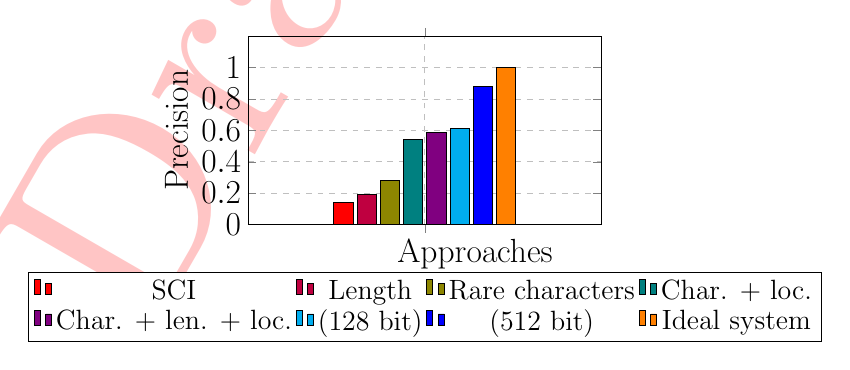
\begin{tikzpicture}[scale=0.7]
  \begin{groupplot}[label style={font=\LARGE},
    	tick label style={font=\LARGE},
% 		xlabel={Approaches},
% 		ylabel={FP},
% 		label style={font=\large},
% 		tick style={font=\large},
		legend style={legend columns=4,at={(0.5,-0.25)},anchor=north,font=\Large},
	    x label style={at={(axis description cs:0.5,-0.1)},anchor=north},
		symbolic x coords = {Approaches},
		x tick label style  = {text width=1cm,align=center},
		xtick=data,
		ybar,
% 		x=5.0cm,
        width = 8cm,
        height = 5cm,
% 		bar width=5.0pt,
		ymin=0.0,
% 		ymode = log,
		ymax=1.2,
		ytick={0.0, .2, .4, .6, .8, 1},
		xmajorgrids=true,
		ymajorgrids=true,
		grid style=dashed ]
    \nextgroupplot [ylabel={Precision}]

%         \addplot[fill=red] coordinates{(Approaches, 0.14)}; \addlegendentry{SCI}
% 		\addplot[fill=purple] coordinates{(Approaches,0.21)}; \addlegendentry{Length}
% 		\addplot[fill=olive] coordinates{(Approaches,0.31)}; \addlegendentry{Rare characters}
% 		\addplot[fill=teal] coordinates{(Approaches,0.58)}; \addlegendentry{Char. + loc.}
% 		\addplot[fill=violet] coordinates{(Approaches,0.63)}; \addlegendentry{Char. + len. + loc.}
% 		\addplot[fill=cyan] coordinates{(Approaches,0.65)}; \addlegendentry{\hash (128 bit)}
% 		\addplot[fill=blue] coordinates{(Approaches,0.89)}; \addlegendentry{\hash (512 bit)}
% 		\addplot[fill=orange] coordinates{(Approaches,1.0)}; \addlegendentry{Ideal system}


        \addplot[fill=red] coordinates{(Approaches, 0.14)}; \addlegendentry{SCI}
		\addplot[fill=purple] coordinates{(Approaches,0.19)}; \addlegendentry{Length}
		\addplot[fill=olive] coordinates{(Approaches,0.28)}; \addlegendentry{Rare characters}
		\addplot[fill=teal] coordinates{(Approaches,0.54)}; \addlegendentry{Char. + loc.}
		\addplot[fill=violet] coordinates{(Approaches,0.59)}; \addlegendentry{Char. + len. + loc.}
		\addplot[fill=cyan] coordinates{(Approaches,0.61)}; \addlegendentry{\hash (128 bit)}
		\addplot[fill=blue] coordinates{(Approaches,0.88)}; \addlegendentry{\hash (512 bit)}
		\addplot[fill=orange] coordinates{(Approaches,1.0)}; \addlegendentry{Ideal system}
    
  \end{groupplot}
\end{tikzpicture}
% \vspace{-.2cm}
\caption{The influence of \hash components on Precision.}
\label{fig:components}
%\vspace{-.2cm}
\end{figure}
We now evaluate the impact of each feature used in \hash on the average precision and the FP rate of \system.
We use the WT (100) datasets in this experiment with the same setup as in the previous experiments.
According to the results in Figure~\ref{fig:components}, encoding the \textit{character and its location} has higher filtering power than the \textit{length} feature.
The difference between \hash and \textit{character + length + location} is the rotation operation.
In particular, we observe that the rotation filters $20\%$ of the remaining FPs undiscovered in \textit{character + length + location}.
This shows that the rotation plays an important role in pruning FPs.

\subsubsection{Join-Key Size}
\begin{figure}[t!]
% \vspace{-.2cm}
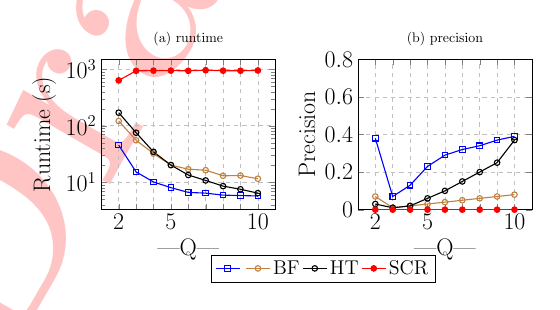
\begin{tikzpicture}[scale=0.5]
  \begin{groupplot}[xtick=data, group style={group size=2 by 1 , horizontal sep=1.0cm}, width = 10cm, every node near coord/.append ,nodes near coords, point meta=explicit symbolic, log origin=infty]%style={yshift=-0.21cm}
    % baseline
    % TR
    % AugX
    
    \nextgroupplot [title = (a) runtime,
    	xlabel={|Q|},
    	ylabel={Runtime (s)},
    	label style={font=\LARGE},
    	tick label style={font=\LARGE},
    % 	legend style={font=\LARGE},
    	legend style={legend columns=2,at={(0.5,-0.2)},anchor=north,font=\Large},
    	width = 6cm,
    	height = 5.4cm,
    	xmin=1,
    	xmax=11,
    	ymin= 0,
    	ymax=1500,
    % 	log basis x={2},
    % 	log basis y={10}, 
    % 	xticklabels={1, , 5,,,,15,,,},
        every axis plot/.append style={thick},
    	ymode=log,
    	xtick={2, 3, 4, 5, 6, 7, 8, 9, 10},
    	ytick={0, 1, 10, 100, 1000},
    	xticklabels={2,,,5,,,,,10,,,,,15},
    	xmajorgrids=true,
    	ymajorgrids=true,
    % 	legend style={at={(1.4,0.7)},anchor=north,font=\LARGE},
    	grid style=dashed]
    	\addplot[color=blue,mark=square] coordinates{(2, 45.4)(3, 15.2)(4, 10.1)(5, 8)(6, 6.6)(7, 6.4)(8, 5.9)(9, 5.8)(10, 5.7)};% \addlegendentry{\hash}
    	\addplot[color=brown,mark=o] coordinates{(2, 121.4)(3, 55.2)(4, 32.2)(5, 20.1)(6, 16.97)(7, 16.3)(8, 13)(9, 13.1)(10, 11.52)}; %\addlegendentry{BF}
    	\addplot[color=black,mark=o] coordinates{(2, 170.1)(3, 75.2)(4, 34.5)(5, 20.1)(6, 13.4)(7, 10.74)(8, 8.52)(9, 7.5)(10, 6.4)}; %\addlegendentry{HT}
        \addplot[color=red,mark=*] coordinates{(2, 634.8)(3, 938.5)(4, 945.9)(5, 946.1)(6, 938.6)(7, 962.3)(8, 943.1)(9, 939.9)(10, 952.1)}; %\addlegendentry{DXF}

    \nextgroupplot [title = (b) precision,
    style={xshift=1.1cm},
    	xlabel={|Q|},
    	ylabel={Precision},
    	label style={font=\LARGE},
    	tick label style={font=\LARGE},
    % 	legend style={font=\LARGE},
    	legend style={legend columns=5,at={(-0.2,-0.3)},anchor=north,font=\Large},
    	width = 6cm,
    	height = 5.4cm,
    	xmin=1,
    	xmax=11,
    	ymin= 0,
    	ymax=.8,
    % 	log basis x={2},
    % 	log basis y={10}, 
    % 	xticklabels={1, , 5,,,,15,,,},
        every axis plot/.append style={thick},
    % 	ymode=log,
    	xtick={2, 3, 4, 5, 6, 7, 8, 9, 10},
    	ytick={0, .2, .4, .6, .8, 1},
    	xticklabels={2,,,5,,,,,10,,,,,15},
    	xmajorgrids=true,
    	ymajorgrids=true,
    % 	legend style={at={(1.4,0.7)},anchor=north,font=\LARGE},
    	grid style=dashed]
    % 	\addplot[color=orange,mark=x] coordinates{(2, 6680)(3, 221)(4, 217)(5, 217)(6, 217)(7, 217)(8, 217)(9, 217)(10, 217)}; \addlegendentry{True positives}
    % 	\addplot[color=blue,mark=square] coordinates{(2, 17587)(3, 3097)(4, 1618)(5, 955)(6, 741)(7, 677)(8, 634)(9, 582)(10, 563)}; \addlegendentry{\hash}
    % 	\addplot[color=brown,mark=o] coordinates{(2, 92883)(3, 23341)(4, 10699)(5, 6440)(6, 5017)(7, 3988)(8, 3483)(9, 3142)(10, 2854)}; \addlegendentry{BF}
    % 	\addplot[color=black,mark=o] coordinates{(2, 211800)(3, 33132)(4, 9645)(5, 3561)(6, 2062)(7, 1405)(8, 1062)(9, 868)(10, 586)}; \addlegendentry{HT}
    %     \addplot[color=red,mark=*] coordinates{(2, 1958951)(3, 1958951)(4, 1958951)(5, 1958951)(6, 1958951)(7, 1958951)(8, 1958951)(9, 1958951)(10, 1958951)}; \addlegendentry{DXF}
        
    	\addplot[color=blue,mark=square] coordinates{(2, .38)(3, .07)(4, .13)(5, .23)(6, .29)(7, .32)(8, .34)(9, .37)(10, .39)}; \addlegendentry{\hash}
    	\addplot[color=brown,mark=o] coordinates{(2, .07)(3, .01)(4, .02)(5, .03)(6, .04)(7, .05)(8, .06)(9, .07)(10, .08)}; \addlegendentry{BF}
    	\addplot[color=black,mark=o] coordinates{(2, .03)(3, .01)(4, .02)(5, .06)(6, .1)(7, .15)(8, .20)(9, .25)(10, .37)}; \addlegendentry{HT}
        \addplot[color=red,mark=*] coordinates{(2, 0)(3, 0)(4, 0)(5, 0)(6, 0)(7, 0)(8, 0)(9, 0)(10, 0)}; \addlegendentry{SCR}
		
  \end{groupplot}
\end{tikzpicture}
% \vspace{-.2cm}
\caption{Key size experiment.}
\label{fig:keysize}
\end{figure}
Here, we evaluate the scalability of \system in the existence of different join-key sizes, i.e.,~the number of columns in the composite key of the input table. 
Due to the limited number of tables with high dimensional composite key, we ran this experiment with a random dataset from the German Open Data corpus with up to 10 columns that can form a composite key (out of 33 columns).
Figure~\ref{fig:keysize} (a) and \ref{fig:keysize} (b) depict the runtime and precision results for different key sizes.
Increasing the number of columns, we observe that the runtime for \system constantly reduces because the FP rate constantly decreases. However, this does not imply a constant increase in precision because increasing the number of key columns changes the ratio of joinable and non-joinable rows. In our experiment, moving from a composite key with two columns to a three-column key, $97\%$ of the joinable rows become non-joinable due to the newly introduced key column. Thus, the filter is confronted with a larger number of FPs, some of which come through.
From key size $4$ upwards, precision increases again as expected.
The runtime gain for larger key sizes is because of two reasons:
\textit{(1)}  With more columns in the query join key, there will be more 1-bits in the query super key, which makes it harder to mask. 
\textit{(2)} Increasing the size of the composite key leads to fewer joinable table rows. Therefore, it is more likely that the second table filtering rule drops the candidate tables without evaluating the remaining rows.
%Again, \hash outperforms other baselines in runtime and precision.   

\subsubsection{Initial column selection.}
%\begin{table}[]
    \small
    \centering
    \caption{Initial query column selection experiment.}
    % \vspace{-.2cm}
    \label{tab:ICS}
\begin{tabular}{l|l|l|l|l|l}
&\textit{\textbf{Best}} & \textit{\textbf{\system}} & \textit{\textbf{Column Order}} & \textit{\textbf{TLS}} & \textit{\textbf{Worst}} \\ \toprule

AVG PL size & 83 & 179 & 202 & 246 & 728

\end{tabular}
\end{table}

We evaluate our heuristic to select the initial query column by comparing the number of retrieved PL items in \system to four other baselines:
\textit{(i)} The column order. In this approach, the initial column will be the first query column according to the column order inside the table. %The idea behind this strategy is that usually, the identifying columns come earlier in the table.
\textit{(ii)} The longest string (TLS). In this approach, the system selects the column that contains the longest cell value as the initial column. %The heuristic here is that the longer the text, the more specific is the column. 
\textit{(iii)} The worst-case scenario. A hypothetical approach that always picks the worst column that returns the larger number of PL items.
\textit{(iv)} Best, i.e. ground truth, which chooses the column that filters most.
The best- and the worst-case scenarios provide lower and upper bounds for our experiment.
This experiment is done using the OD (10k) tables.
In this experiment our cardinality-based heuristic outperfmed the other heuristics. It retrieved on average only 179 PLs compared to Column Order, TLS, and the worst-case scenario with 202, 248, and 728 Pls, respectively. The optimal number of PLs based on ground truth was 83. The heuristic used in \system performs better because of the fact that the number of PL items per cell value follows the power-law distribution. There is a small set of values that have a large number of PL items but most of the values lead to a similar number of PL items (The average number is $12$).
%Table~\ref{tab:ICS} shows that the cardinality-based heuristic used in \system, performs best and is very close to the ground truth approach. The heuristic used in \system performs better because of the fact that the number of PL items per cell value follows the power-law distribution. There is a small set of values that have a large number of PL items but most of the values lead to a similar number of PL items (The average number is $12$).% Thus, there is a direct relationship between the cardinality and the number of retrieved PL items.





\textbf{Related work}:
% Object detection related datasets/algo in non-medical domain
% Locally labeled CXR dataset
A few CXR datasets have localized abnormality annotations \cite{shih2019augmenting,filice2020crowdsourcing,jaeger2014two} that are curated manually. These are high quality gold standard ground truth datasets but tend to be smaller in scale (< 30,000 images) and have a narrow coverage, with typically only 1-2 labels. In addition, since most labeling efforts only have abnormality semantics attached, no direct relationships with the affected anatomical locations are available. 

%MEHDI: repeated concepts from above. I am removing the following: 

%The lack of anatomic semantics in the annotation is a limitation for complex multi-modal clinical reasoning work, e.g., differential diagnosis, since clinicians often integrate information along anatomical lines, and for downstream report generation tasks, which often requires describing not only the abnormality but also correctly communicate the location of the abnormalities (and medical devices) to the receiving clinicians. 

Two recent CXR datasets have labels for anatomies described in the reports. In \cite{datta2020dataset}, a small manually annotated dataset (2000 reports) included 10 abnormalities that are individually associated with 29 unique spatial locations (anatomies) at the report level. Another CXR dataset has automatically extracted abnormality and anatomy labels as disconnected concepts that are only correlated at the study level from  160,000 reports using a supervised NLP algorithm \cite{bustos2020padchest}. This was trained on a smaller set of manually annotated data. Neither datasets contain localized annotations for the associated CXR images, nor any comparison relation annotations between sequential exams, both of which are available in the Chest ImaGenome dataset. In Table \ref{tab:related}, we present a comparison of our Chest ImagGenome dataset with other datasets available in the literature.

% Table -- Kashyap

% MEdical imaging datasets to go here: Discussed that we will only focus on cxr datasets that are available for this paper. 
% \caption{\color{red} Kashyap, feel free to continue with the table. We should remove the questionmarks and add a line for our dataset (since all others are not graph). For longer text, using abbreviations and explaining them in the caption often works better. If fill in the values is not possible, it is better to remove the table altogether.}


\begin{table}[t!]
\caption{Summary of existing chest X-ray datasets}
\resizebox{\textwidth}{!}{%
\begin{tabular}{@{}lllllllll@{}}
\toprule
\textbf{Dataset} & \textbf{Annotation Level} & \textbf{Annotation Method} & \textbf{Num Labels} & \textbf{Anatomy Labeled} & \textbf{Graph} & \textbf{Dataset Size} & \textbf{Temporal Labels} & \textbf{Reports} \\ \midrule
SIIM-ACR Pneumothorax Segmentation \cite{filice2020crowdsourcing} & Segmentation & Manual + augmented & 1 & No & No & 12,047 & No & No \\
RSNA Pneumonia Detection Challenge   \cite{shih2019augmenting} & Bounding Boxes & Manual & 1 & No & No & 30,000 & No & No \\
Indiana University Chest X-ray collection \cite{demner2016preparing} & Global & Automated & 10 & No & No & 3,813 & No & Yes \\
NIH CXR dataset \cite{wang2017chestx} & Global & Automated & 14 & No & No & 112,120 & No & No \\
PLCO \cite{team2000prostate} & Global & Automated & 24 & Yes & No & 236,000 & Yes & No \\
Stanford CheXpert \cite{irvin2019chexpert} & Global & Automated & 14 & No & No & 224,316 & No & No \\
MIMIC-CXR \cite{johnson2019mimic} & Global & Automated & 14 & No & No & 377,110 & No & Yes \\
Dutta \cite{datta2020dataset} & Global & Manual & 10 & Yes & Yes & 2,000 & No & Yes \\
PadChest \cite{bustos2020padchest} & Global & Manual + automated & 297 & Yes & No & 160,868 & No & Yes \\
Montgomery County Chest X-ray   \cite{jaeger2014two} & Segmentation & Manual & 1 & Yes & No & 138 & No & No \\
Shenzen Hospital Chest X-ray   \cite{jaeger2014two} & Segmentation & Manual & 1 & Yes & No & 662 & No & No \\  \hline \hline
\textbf{Chest ImaGenome} & Bounding Boxes & Automated & 131 & Yes & Yes & 242,072 & Yes & Yes \\
\bottomrule
\end{tabular}%
}
\label{tab:related}
\vspace{-0.4cm}
\end{table}
% removed (Derived from MIMIC-CXR \cite{johnson2019mimic}) % makes table really small

\section{Conclusion and Future Work} \label{sec:conclusion}
In this paper, we tackled the problem of n-ary or multi-attribute join search. We proposed a hash-based filtering approach \system that removes redundant table rows from further joinability calculation processes to increase the scalability of the join discovery. We proposed \hash, a hash function that leverages syntactic features of the cell values that ultimately lead to the lowest FP rates. We showed that \system is more effective and efficient than state-of-the-art systems.
We focused on the equi-joins. Because \hash uses syntactic features including the character and length features of the cell values, it has the potential to discover similarity joins as well. According to our observations, the false positives caused by \hash were those that are syntactically similar to the actual key values, e.g., discovering the composite key <``brooklyn'', ``cambridge''> instead of <``brooklyn'', ``bay ridge''>. 
Another future direction is to reason about hashing short key values. \hash cannot use its optimal potential if cell values are too short.


\begin{acks} 
This project has been supported by the German Research Foundation (DFG) under grant agreement 387872445 and the German Ministry for Education and Research as BIFOLD — “Berlin Institute for the Foundations of Learning and Data” (01IS18025A and 01IS18037A).
\end{acks}

\balance

% \small
%\bibliographystyle{abbrv}
 \bibliographystyle{ACM-Reference-Format}
\bibliography{references}

\end{document}
